% Created 2021-04-15 Thu 15:11
% Intended LaTeX compiler: pdflatex
\documentclass[11pt]{article}
\usepackage[mathletters]{ucs}
\usepackage[utf8]{inputenc}
\usepackage[T1]{fontenc}
\usepackage{graphicx}
\usepackage{grffile}
\usepackage{longtable}
\usepackage{wrapfig}
\usepackage{rotating}
\usepackage[normalem]{ulem}
\usepackage{amsmath}
\usepackage{textcomp}
\usepackage{amssymb}
\usepackage{capt-of}
\usepackage{hyperref}
\usepackage[backend=biber,style=apa,natbib=true]{biblatex}
\addbibresource{/home/joe/My Library.bib}
\usepackage[a4paper,bindingoffset=0.2in,left=1in,right=1in,top=1in,bottom=1in,footskip=.25in]{geometry}
\usepackage[dvipsnames]{xcolor}
\usepackage{fontspec}
\usepackage[math-style=french]{unicode-math}
\usepackage{mathtools}
\setmathfont[math-style=upright]{DejaVu Sans Mono}
\setmonofont[scale=.8,Color=blue]{Ubuntu Mono}
\newfontfamily{\mm}[scale=.8,Color=red]{DejaVu Sans Mono}
\setmainfont[BoldFont=EB Garamond,BoldFeatures={Color=ff0000}]{EB Garamond}
\newcommand{\hookuparrow}{\mathrel{\rotatebox[origin=c]{90}{$\hookrightarrow$}}}
\usepackage{fix-abstract}
\definecolor{pale}{HTML}{fffff8}
\definecolor{orgone}{HTML}{83a598}
\definecolor{orgtwo}{HTML}{fabd2f}
\definecolor{orgthree}{HTML}{d3869b}
\definecolor{orgfour}{HTML}{fb4933}
\definecolor{orgfive}{HTML}{b8bb26}
\definecolor{gruvbg}{HTML}{1d2021}
\newenvironment*{emptyenv}{}{}
\usepackage{sectsty}
\sectionfont{\normalfont\color{red}\selectfont}
\subsectionfont{\normalfont\selectfont}
\paragraphfont{\normalfont\selectfont}
\subsubsectionfont{\normalfont\selectfont\color{black!50}}
\author{Joe Corneli}
\date{\today}
\title{Hyperreal Enterprises: Roadmap}
\hypersetup{
 pdfauthor={Joe Corneli},
 pdftitle={Hyperreal Enterprises: Roadmap},
 pdfkeywords={},
 pdfsubject={},
 pdfcreator={Emacs 28.0.50 (Org mode 9.4.4)}, 
 pdflang={English}}
\begin{document}

\maketitle
\begin{abstract}
\noindent This document can be thought of as an informal outline of a “\emph{tactic state}”.  On a technical level, the upstream source for this material is an Org Roam graph.  The “Wiki” section contains instructions for accessing the material and generating derived formats, such as the Org Agenda.
\end{abstract}

\setcounter{tocdepth}{2}
\tableofcontents
\section{Hyperreal Enterprises: Roadmap}
\label{sec:org1dd8ae1}

\subsection{Preface}
\label{sec:org5ce2cb8}
This document synthesises a \href{http://www.peeragogy.org/pattern-roadmap.html}{Roadmap} (and perhaps also a \href{http://scrumbook.org/value-stream/product-roadmap.html}{Product
Roadmap}) for Hyperreal Enterprises, Ltd.  The Roadmap is being written
inside \href{https://github.com/org-roam/org-roam}{Org Roam} (an \href{https://www.gnu.org/software/emacs/}{Emacs} package), and displayed with \href{https://github.com/theiceshelf/firn}{Firn}.  The
document can be thought of as a \hyperref[sec:org675d604]{Wiki} (and edited inside Emacs).  From
these sources, other downstream formats can be derived.  A narrative
introduction follows.

To skip it, browse ahead to \hyperref[sec:org7f060ab]{Top}.

\subsection{Introduction}
\label{sec:org226b341}

\subsubsection{Applying AI to technical fields is a huge opportunity.}
\label{sec:org0228c7c}

It’s striking that in computer programming work, \emph{collective
intelligence} is used almost everywhere, but artificial intelligence is
used almost nowhere.  AI can kick butt at Chess and Go, but university
courses are still taught by human professors.  Surely, AI that could
write code at a human level would be a valuable thing\ldots{}

\subsubsection{But where’s the human-level AI for coding?}
\label{sec:org3fd9cf6}

A research agenda around “AI for programming” was already spelled out
by Alan Turing in the late 1940s.  It is only relatively recently that
we have massive amounts of relevant data to work with.  Code
completion and code generation tools are some of the “low hanging
fruit” of this domain.  We think that something much more substantial
is around the corner.

\subsubsection{We are looking at this problem as an informal open source R\&D collective.}
\label{sec:org38d4faf}

Our loose-knit team brings together applied experience in Natural Language
Processing (NLP), computational modelling, online communities,
mathematical sciences (\(x!\)) as well as humanities and social science.  We’ve been getting
together for daily coffee chats, and sharing information and skills
with each other in online seminars.  Sometimes we bring in guest
speakers.  We hope as time goes by our chats will coalesce into notes,
blog posts, papers, and working prototypes.  We aren’t promising a
schedule of deliverables — because we’re all volunteers — and we’re
doing this for fun and interest.  But we do plan to share what we’re
learning as we go along!

\subsubsection{Broadly, the steps we have in mind go from data, to models, to AI agents.}
\label{sec:org459165a}

We plan to document our progress (or lack thereof) on this blog.  As a
very rough outline, this is what we expect to look at:

\begin{itemize}
\item We plan to use contemporary information extraction methods to derive computationally meaningful material from Stack Exchange Q\&A, Github Issues, and programmers’ discussions, along with code. To do this, we will combine general purpose language models, like BERT, and a knowledge graph approach.

\item We plan to use category theoretic methods as a glue that can hold together a range of computational models, including models of programs and the process of computer programming. \href{https://arxiv.org/pdf/1807.05691}{Monocl} is an existing process modelling language that has been used to create an abstraction layer over a collection of \href{https://www.datascienceontology.org/}{data science programs}. We plan to generalise this.

\item Ultimately, we plan to install these models in computational agents who can then “converse with each other to sharpen their wits,” as Turing anticipated, mirroring contemporary developments in self-play.  However, the specific design of the agents remains an open issue at the moment!  We plan to explore techniques from Bayesian learning, logic programming, and reinforcement learning.
\end{itemize}

\subsubsection{Reflection is part of the process.}
\label{sec:org9cf84d5}

We’re interested in understanding human behaviour as well as technical
topics: that goes for our own behaviour in particular.  We plan to
post to our blog at least monthly — as long as we keep our discussion
running — using it as a place to reflect on how things are going.
Although we’re grappling with some weighty topics, success is not all
or nothing!  Writing here will mark our progress and be useful in
their own right (e.g., blog posts can feed into research papers or
tools).

\subsubsection{Progress so far}
\label{sec:org34f617c}
Alongside setting up a blog and drafting an initial anouncement
(voilà!), we’ve updated the website of our affiliated UK-based company
\href{https://hyperreal.enterprises/}{Hyperreal Enterprises} to match the outlines of what we’ve described
here.  As mentioned above, are having regular meetings, which we’ll
record if they look likely to be interesting to a wider audience.
We’ve got nice internal documentation going, via \href{https://github.com/org-roam/org-roam}{Org Roam}, from wich
various derived formats are produced, including a public \href{https://exp2exp.github.io/}{wiki}
generated by \href{https://github.com/theiceshelf/firn}{Firn}.  (We recently sent an abstract to EmacsConf 2020 to
talk about the various other Emacs-based tools we’re using!)

Some of our seminars so far have explored an Open Information
Extraction (with several demo notebooks), and looked at the early
parts of Michael Betancourt’s “Towards a principled Bayesian
workflow”.

Active channels on our Discord server include:
\begin{itemize}
\item \#emacs-cloud-hypernotebooks
\item \#how-to-design-programs
\item \#text-analysis
\item \#model-construction
\item \#knowledge-graph
\end{itemize}

\subsubsection{TL;DR}
\label{sec:orgf4979c0}

We are creating AI tools that will process open source information and
build on these in applications such as automated programming.

\section{Top}
\label{sec:org7f060ab}
\subsection{Motivation: For the sake of advancing AI}
\label{sec:org31b7a62}
We are doing this R\&D work partly to make demonstrations of more
advanced AI systems.  We expect that our stance on AI will not
necessarily be a popular one.  But this is an important “minor” strand
of AI research dating back to Alan Turing:

\begin{quote}
``As time goes on the [computer] itself will take over the functions
both of [programmers] and of [users]…The [programmers] are liable to
get replaced because as soon as any technique becomes at all
stereotyped it becomes possible to devise a system of instruction
tables which will enable the electronic computer to do it for
itself. It may happen however that the [programmers] will refuse to do
this. They may be unwilling to let their jobs be stolen from them in
this way. In that case they would surround the whole of their work
with mystery and make excuses, couched in well chosen gibberish,
whenever any dangerous suggestions were made.'' -- Alan Turing, 1947.
\end{quote}

On average, advanced AI would bring in new ways of working, and would
facilitate broad access to high-quality training.  This agenda could
serve to focus the mind of technical workers, but not many are
pursuing it presently.

\subsection{Motivation: Technical experiments become easier}
\label{sec:org2270e8f}

Even in the present time, without relying on any speculative AI
futures to magically appear, we can benefit from pursuing the agenda
above.  Accordingly, we are doing some applied work with existing
software that will give us a set of further tools and levers to work
with.

\subsection{Representative Prior Work}
\label{sec:org2aabcc0}

\subsubsection{PlanetMath}
\label{sec:orgec3998f}

\href{https://planetmath.org/}{PlanetMath} users created a reasonably large informal mathematical
knowledge base together.  On the way, we came up with several
technical demos and sketched possible \href{https://github.com/holtzermann17/planetmath-docs/labels/PREVIEW}{previews} for upcoming features.
One possible direction of work we looked at would be to focus on
building a comprehensive category theory knowledge base.

\subsubsection{Modelling the way mathematics is actually done}
\label{sec:org1a58d09}

In \href{https://www.newton.ac.uk/files/preprints/ni17003.pdf}{this paper}, we talked about how mathematics is situated somewhere
in between ‘games’ and ‘storytelling’ in its complexity.  We proposed
to build computational models of informal mathematical reasoning.
Subsequent work continued on in this direction, using ideas from
\href{https://www.sciencedirect.com/science/article/pii/S0004370217300267}{dialogue games} and \href{https://link.springer.com/article/10.1007/s10503-018-9474-x}{argumentation theory more broadly}.

\subsection{A sketch of a plan}
\label{sec:org7a3746f}

So, having gotten together around these ideas, we’re having online
chat, frequent short meetings.  We’ve talked about maintaining a blog
that would describe what we’re learning and developing.  So, roughly
speaking, we will try to develop a curriculum through the blog.  We
also have this wiki, that any of us can edit, which we can use as a
staging ground for more developed blog posts.  Our thought was that
blog posts might move in the direction of more developed outputs,
whether products or research papers.  We want to use some ideas
adapted from Scrum to build a shared awareness of what’s going on.
However, we want to be careful not to become “managerial” since
everyone is currently here as a volunteer, working on topics of his or
her own interest.  We want to provide mutual support and fun.
Reflection, whether in writing, or by recording and listening again to
conversations, should help with that.  We are not constraining things
to come out in a purely structured curriculum, or any other form of
product development.  “Users” and “customers” may appear as we release
things we are happy with and expand our little community.

\begin{quote}
“Rousseau says, someone who has been properly educated will be engaged
in society, but relate to his or her fellow citizens in a natural way.
\ldots{} We naturally look after our own
preservation and interests.  By contrast, \emph{amour-propre} is an unnatural
self-love that is essentially relational. \ldots{} Thus, \emph{amour-propre} can
contribute positively to human freedom and even virtue. Nevertheless,
\emph{amour-propre} is also extremely dangerous because it is so easily
corruptible. \ldots{} In its corrupted form, \emph{amour-propre} is the source of
vice and misery, and results in human beings basing their own self
worth on their feeling of superiority over others.” — \href{https://iep.utm.edu/rousseau/}{IEP}
\end{quote}

\subsection{A possible formulation: short correlated sprints as opposed to random behaviour}
\label{sec:org3c9368d}

“Two people working together 4 hours a week for two weeks” could serve
as an approximate unit of work.  Once we have amassed a few outputs
from this kind of effort, we will have some evidence of the kinds of
things that we can realistically achieve.  So far, our workflow has
been more based on solo activities and informal conversations, but
short robust team-ups continue to be an option!

\begin{quote}
Hypothetical conversation: \emph{In my next post I want to integrate something that I learned from you about PL.  I want to drive in the direction of synthesis, as hard as I know how to right now.  This depends on everyone having free time to invest in this.  Start a blog where we think about what's the overlap in terms of learning?}
\end{quote}
\section{Why not what}
\label{sec:org2ebea07}
Our purpose:

\begin{itemize}
\item We want to make the knowledge economy accessible to everyone.
\item Our long-term vision is computational intelligence based on collective intelligence.
\end{itemize}
\subsection{Teach arbitrary coding}
\label{sec:org3fd6966}
This would be an abstraction over teaching basic programming and
knowledge graphs.

\subsubsection{Feature: Production system}
\label{sec:org27f51e2}

We’ve started to build a simple production system that can be used to
detect errors in subtraction (reimplementing some classic work). We
were thinking that something similar could be used to detect other
kinds of errors (so, for debugging, teaching), and to support other
kinds of reasoning processes (e.g., turning Q’s into A’s in a
question-answering system).

We previously did a little exploratory work, with similar intent, using
polygraphs as input, in the workshop paper
\emph{Modelling the Way Mathematics Is Actually Done}.

\begin{enumerate}
\item Demo application: Reimplementing classic rules to model subtraction
\label{sec:orgd17f6e1}

We looked at a classic paper about “subtraction on Mars” and it seems
that reimplementing it might be the best way to go.
\end{enumerate}

\subsection{How to Design Programs}
\label{sec:orgfce34d0}
We were thinking of \emph{How to Design Programs} (HtDP) as a potential
basis for this work.  We would want to respect category theoretic
concepts in the presentation.  We would expect to find analogues in
settings like Bayesian modelling.

We could proceed by looking at relationships with argumentation
theory, thinking about how to do this in a theoretically consistent
way.  Once we have a definition of the programming language we’re
going to use, we can then do argumentation over that.

Another strategy would be to develop a DSL for HtDP ideas, which we
could then reuseq to generate patterns for learning how to design
various structures (say, web pages or probabilistic programs).  To do
this well you’d need ways to express ‘recipes’.  For example, an MVP
might be based on representing HtDP-style recipes using sequent
calculi for session types.  These represent interactive protocols.

You’d use cut-elimination to have two players interact (using
something like the \textbf{\textbf{Lakatos Game diagram}}).  But what formalism
would you use?  E.g., \emph{geometry of interaction in linear logic} has
been used for this kind of thing, but could it be used here?  With a
suitable formalism in place we would then imagine that a computer
programming agent would just follow the “Lakatos Game” style HtDP
script.  So, this would contribute to the development of agent models
for programming and program-related Q\&A.

\subsubsection{Related work}
\label{sec:org7338c21}

\begin{itemize}
\item General theory-informed algorithms (e.g., apply category theory to scientific models).
\item K framework: Have transformations for any language you define in it.
\item HtDP is similar applied to programming teaching.  Start with PL theory and then find universal things.
\item How can we define statistics in a general way and then derive things from it?  (E.g., Anglican probabilistic programming?)
\end{itemize}
\section{Construct, critique, improve models of the creative process}
\label{sec:orgf317374}
We want tools and processes for working with models, with a particular
emphasis on improved models of the creative process. The reason for
this emphasis is that if we have good models of the creative process,
including the modelling process, we can then apply them to a wide
range of problems!  This prompts reflection on the infrastructure and
tools that we are actually using.

\subsection{Emacs Hyper Notebook}
\label{sec:orgded891b}
We are developing a better way to do “Jupyter notebooks” using Emacs.
This recovers some of the Research Collab ideas developed by Aaron
Krowne. It should integrate features such as writing and task
management (e.g., \emph{Org}) Program evaluation (e.g., \emph{Maxima}),
Typesetting and presentation (e.g., slides via \emph{\LaTeX{}}), and
navigation (e.g., \emph{Org Roam} for displaying topics as a graph).  We
should be clear that the various technologies used are slot-fillers
and they might be replaced with other things, or augmented (e.g.,
\emph{Lean} for formal verification of some of the above?). A useful input
to this process would be implementation of examples without
integration.  This can then be redone in a more integrated fashion.

An integration using existing technologies will have limitations, once
we have this demos then we will see some of the gaps and how more
advanced tech could be useful. (For example, Ray’s work with Gerschom
could turn out to be useful here.)

\begin{enumerate}
\item Some quick thoughts
\label{sec:org0b91668}

\begin{itemize}
\item If it was sitting inside a web container, then maybe it’s a quickstart thing that comes in a user friendly form.
\item Maybe add menu-bar items to make it look like a web browser.
\item Emacs Maxima interface, we might build on it — for Monday 12th October, a quick ``15 minutes'' talk to catch up
\item \ldots{} possible deliverable for later on: a NIST talk?
\end{itemize}
\end{enumerate}

\subsubsection{{\bfseries\sffamily DONE} Figure out subtasks to deliver for EmacsConf\hfill{}\textsc{joe:ray:cameron}}
\label{sec:org9b48467}
\subsubsection{{\bfseries\sffamily BACK} Figure out how EHN relates to other projects}
\label{sec:org132c19d}
\subsubsection{{\bfseries\sffamily DONE} Keep testing crdt.el and lockstep.el\hfill{}\textsc{joe:ray}}
\label{sec:org5207371}
\subsubsection{{\bfseries\sffamily BACK} Could Emacsconf talk become a blog post?\hfill{}\textsc{joe:ray:cameron}}
\label{sec:orgebc28da}

(Notice that with crdt, typing can go on inside folded nodes! Qiantan
is thinking about a mode to make overlays shareable, which would
change things a bit.)

\subsubsection{Partial prototypes}
\label{sec:orgcfe9eec}

How far can we go\ldots{} Through \href{https://roamresearch.com/}{Roam}? (We could at least talk to Connor
about Roam on Twitter?) Through \href{https://jupyter.org/}{Jupyter}? \href{https://foambubble.github.io/foam/}{Foam}? \href{https://gtoolkit.com/}{Glamorous Toolkit}?  Can
we integrate what we’re building with existing tools like these?  Do
Lenses or other kinds of ACT machinery help with this at all?  Would
our system potentially play a role as a universal backend?

\subsubsection{Feature: Arxana 2020}
\label{sec:orgc729a59}

Revisit \href{https://repo.or.cz/w/arxana.git}{Arxana} and turn it into something that we can actually use.
This is rather closely related to the use of “knowledge graph”
formulations we’ve been discussing, since Arxana allows us to combine
writing with knowledge representations.  In our last round of work
with Arxana, we left off at the point of integrating logic programming
into the system.

\subsubsection{Links to useful resources}
\label{sec:org2130255}

Technology like this could be used to build simple demos (e.g., Emacs
in the browser, running Org Mode).  We’ve noticed some other related
tools as well, like \href{https://github.com/200ok-ch/organice}{Organice} and \href{https://github.com/tecosaur/codiorg}{CodiOrg} that could provide
alternative interfaces.

\begin{itemize}
\item \href{https://github.com/exp2exp/notebooks}{exp2exp/notebooks: This is a Docker configuration for running jupyter with multiple kernels on Arch Linux.}
\item \href{https://www.gnu.org/software/emacs/manual/html\_node/emacs/emacsclient-Options.html}{emacsclient Options - GNU Emacs Manual}
\item \href{https://github.com/butlerx/wetty}{butlerx/wetty: Terminal in browser over http/https. (Ajaxterm/Anyterm alternative, but much better)}
\item \href{https://github.com/xtermjs/xterm.js\#real-world-uses}{xtermjs/xterm.js: A terminal for the web}
\item \url{https://twitter.com/cianbutlerx}
\item \href{https://github.com/tsl0922/ttyd}{tsl0922/ttyd: Share your terminal over the web}
\item \href{https://github.com/yudai/gotty}{yudai/gotty: Share your terminal as a web application}
\item \href{https://hub.docker.com/r/butlerx/wetty}{butlerx/wetty - Docker Hub}
\item \href{https://medium.com/@pacroy/setup-web-terminal-using-wetty-docker-image-dcb1ea75bfaf}{Setup Web Terminal using Wetty Docker Image | by Chairat Onyaem (Par) | Medium}
\item \href{https://hub.docker.com/r/krishnasrinivas/wetty/}{krishnasrinivas/wetty - Docker Hub}
\end{itemize}

\subsubsection{Other related work}
\label{sec:org57c4b24}

\begin{itemize}
\item James Fairbanks (relate this to Betancourt).
\end{itemize}

\subsubsection{Testing}
\label{sec:org736d3e0}

\begin{verbatim}
(def a 2)
\end{verbatim}

\begin{verbatim}
#'user/a
\end{verbatim}

\begin{verbatim}
a
\end{verbatim}

\begin{verbatim}
2
\end{verbatim}

\begin{verbatim}
(range 10)
(def a 1)
\end{verbatim}

\begin{verbatim}
| (0 1 2 3 4 5 6 7 8 9) |
| #'user/a              |
\end{verbatim}

\begin{verbatim}
a
\end{verbatim}

\begin{verbatim}
1
\end{verbatim}

\subsubsection{Implementing a quick demo for Emacs NYC}
\label{sec:orgba3f78d}
Notes for the first talk will appear here:

\begin{itemize}
\item \hyperref[sec:org09289b9]{Hypernotebook First Demo}
\end{itemize}

\subsubsection{What would we actually want as our org interface?}
\label{sec:org78e4516}

We had a short problem with this:

\begin{verbatim}
1+1;
(error "No such language mode: nil-mode")
...
\end{verbatim}

\subsubsection{Backends}
\label{sec:org3a44389}
\begin{enumerate}
\item jupyter
\label{sec:orgd365230}
The jupyter backend works well locally but suffers from a bug when run via tramp. See \hyperref[sec:org3a37c27]{emacs-jupyter remote debugging}

\item ob-streams
\label{sec:org0bbf722}

This is work in progress, with some sample content above.
\end{enumerate}

\subsubsection{Future work}
\label{sec:orgd066cdb}

\begin{itemize}
\item Extending to VS Code?  Would people who use VS code even want this kind of interaction?  Maybe VS Code is better for quick visualisations?
\end{itemize}
\subsection{Hypernotebook First Demo}
\label{sec:org09289b9}

First demo notes will go here.

\subsubsection{During our first session on this, we set up a calculator}
\label{sec:orgdf0047f}

We wrote up a configuration, starting from what the \texttt{src} block might
look like:

\begin{itemize}
\item \texttt{:process} stands in for \texttt{:session} now as an alternative
\item \texttt{org-babel-execute-src-block} this is the function that will be called
\item We saw we had to hang into the \texttt{lang} parameter of the above function, but override using \texttt{:process}
\item The variable \texttt{org-stream-output} needs to be defined (it's in our \texttt{ob-stream.el}).
\item The function \texttt{org-babel-stream} needs to be defined as well (it's in our \texttt{ob-stream.el}).
\item If you're going to use a language mode like \texttt{calc} it should be required.
\item The process itself needs to be defined as well.
\item \texttt{(setq org-confirm-babel-evaluate nil)} should be set.
\end{itemize}

This is an example of what we came up with:

\texttt{\#+begin\_src calc :stream calculator :results output org}

\begin{verbatim}
10*8
\end{verbatim}

\begin{verbatim}
80
\end{verbatim}

\subsubsection{Background research}
\label{sec:org22fc439}

We took a good look at emacs-jupyter to understand how it works.
It seems to work reasonably well but not able to do all the hops via TRAMP to connect with a notebook running on Google Cloud.  This is documented as bug \#191 in the emacs-jupyter repo.

\subsubsection{Now we wanted to improve this to make it more robust}
\label{sec:orgbbb52cf}

\begin{itemize}
\item Be able to handle multiple backends (now via ``servants'' for different shell commands and potentially other processes), not just the \texttt{bc} calculator!
\item In the first version we just used a variable to store things, now use a hash table to organise the data better (\texttt{org-babel-servant-info})
\item Generalise everything
\end{itemize}

\subsubsection{Stitching things together}
\label{sec:org76b6872}

\begin{itemize}
\item Find a good way to weave \texttt{org-babel-servant} into \texttt{org-babel-execute-src-block}
\item Organise the callbacks, can we demo it calling Maxima?
\end{itemize}

\begin{enumerate}
\item Getting things going
\label{sec:org52ce1b8}

\begin{verbatim}
;; Here we start the process
(get-buffer-create "maxima-error")
(setq maxima-proc
      (make-process
       :name "maxima-proc"
       :command '("maxima" "--very-quiet") ;; if we need parameters can add here
       :stderr "maxima-error"
       :filter #'org-stream-string-callback))

(setq calculator-proc
      (make-process
       :name "calculator-proc"
       :command '("bc" "-q") ;; if we need parameters can add here
       ;; :stderr "maxima-error"
       :filter #'org-stream-number-callback))
\end{verbatim}

\begin{enumerate}
\item Calculator example again
\label{sec:orgec0e102}
\begin{verbatim}
10+1
\end{verbatim}

\begin{verbatim}
10
\end{verbatim}

\item Maxima example
\label{sec:org2ad61ec}

Here we call the process we just started.

\begin{verbatim}
3+600000000;
\end{verbatim}

\begin{verbatim}
600000003
\end{verbatim}

\begin{verbatim}
display2d:false;
\end{verbatim}

\begin{verbatim}
false
\end{verbatim}

\begin{verbatim}
expand((x+1)^9)
\end{verbatim}

\begin{verbatim}
$$x^9+9\,x^8+36\,x^7+84\,x^6+126\,x^5+126\,x^4+84\,x^3+36\,x^2+9\,x+1$$
\end{verbatim}

\begin{verbatim}
expand((x+1)^1)
\end{verbatim}

\begin{verbatim}
$$x+1$$
\end{verbatim}
\end{enumerate}
\end{enumerate}

\subsubsection{Ob-servant example}
\label{sec:org91703d6}

\begin{enumerate}
\item Calculator example again
\label{sec:org2d4adec}
\begin{verbatim}
10+1
\end{verbatim}

\begin{verbatim}
11
\end{verbatim}
\end{enumerate}

\subsubsection{Next steps}
\label{sec:org63e5b1c}

\begin{itemize}
\item Change the formatting of the output so it doesn't come across as a table
\item Carry on with ob-servant to integrate it (improve calling Maxima, errors)
\item Raise the change with the Org maintainers
\item Package it up! (patch + repo?)
\item 5 minute talk for Emacs New York (Monday 2 November 2020).
\end{itemize}

\subsubsection{Social Networking}
\label{sec:orgfec9f82}

\begin{itemize}
\item Talk with Fermin to understand what he's doing with Maxima and see if we need to do anything differently
\end{itemize}

\subsubsection{Final polishing}
\label{sec:orge09b3ce}

\begin{itemize}
\item Consider renaming it to ob-servent!
\end{itemize}
\subsection{emacs-jupyter remote debugging}
\label{sec:org3a37c27}
\subsubsection{Debugging}
\label{sec:org0d6f37c}

\begin{enumerate}
\item Initial fix (of what turned out to be a minor problem)
\label{sec:org97107bb}
\begin{itemize}
\item \texttt{jupyter-start-kernel} was problematic, because the id didn’t seem to be set correctly
\begin{itemize}
\item line -2 from end of this function, added \texttt{:id (substring conn-file -41 -5)}.
\end{itemize}
\end{itemize}

\item Ongoing concerns: can we access the kernel?
\label{sec:org331cbec}
\begin{itemize}
\item However, this still doesn’t solve our problem
\begin{itemize}
\item Now we are debugging \texttt{jupyter-kernel-info}
\item Our aim is to figure out \texttt{jupyter-send-kernel-info-request}, maybe also \texttt{jupyter-wait-until-received}
\end{itemize}

\item jupyter-comm-initialize
\item jupyter-kernel-info
\item jupyter-make-client
\item jupyter-session —
\item jupyter-kernel-info — doesn’t get a message back for some reason
\end{itemize}

We suspect it looks at the wrong kernel b/c it examines an id that
doesn’t seem to exist on the server.

\begin{verbatim}
(with-slots (kernel) manager
  (oref kernel session))
\end{verbatim}
\end{enumerate}

\subsubsection{Set up container on gcp}
\label{sec:orgb3fe40f}
\begin{enumerate}
\item gcp configuration
\label{sec:orgd7ba6e3}

You may like to run \texttt{gcloud auth login} ( \href{https://cloud.google.com/sdk/gcloud/reference/auth/login}{auth login docs} ). This is an interactive process that launches oauth for your google account in the web browser so I think it is best to do it from a terminal though it may be possible to run it in org-babel.

\begin{verbatim}
gcloud config configurations list
\end{verbatim}

\begin{verbatim}

NAME     IS_ACTIVE  ACCOUNT                  PROJECT  COMPUTE_DEFAULT_ZONE  COMPUTE_DEFAULT_REGION
default  True       holtzermann17@gmail.com  quarere
\end{verbatim}


\begin{verbatim}
gcloud config configurations describe quarere
\end{verbatim}

\begin{verbatim}
ERROR: (gcloud.config.configurations.describe) The configuration [quarere] does not exist.
\end{verbatim}

\item launch container image
\label{sec:org486ae7c}

Deploy a vm based on the container \texttt{cameronraysmith/notebooks:latest}.

\begin{verbatim}
gcloud compute instances create-with-container notebooks-vm \
    --container-image registry.hub.docker.com/cameronraysmith/notebooks:latest \
    --container-restart-policy on-failure \
    --container-privileged \
    --container-stdin \
    --container-tty \
    --container-mount-host-path mount-path=/home/jupyter,host-path=/tmp,mode=rw \
    --machine-type n1-standard-1 \
    --boot-disk-size 50GB \
    --preemptible
\end{verbatim}

Setup ssh with your new instance

\begin{verbatim}
gcloud compute config-ssh
cat ~/.ssh/config | grep "Host notebooks"
\end{verbatim}

\begin{verbatim}
You should now be able to use ssh/scp with your instances.
For example, try running:
ssh notebooks-vm.us-central1-f.quarere
Host notebooks-vm.us-central1-f.quarere
\end{verbatim}


You can \texttt{ssh} into the host machine or the container using the various commands below.

\begin{verbatim}
gcloud compute ssh notebooks-vm # into host machine
ssh notebooks-vm.us-central1-f.quarere docker ps -aqf "name=klt-notebooks-vm-cjme" # check the container ID
gcloud compute ssh notebooks-vm --container klt-notebooks-vm-cjme # use gcloud ssh with --dry-run to print the command
ssh -t notebooks-vm.us-central1-f.quarere -- sudo docker exec -it klt-notebooks-vm-cjme /bin/sh # this takes you directly into the container
\end{verbatim}

Of course you can stop and start the machine with

\begin{verbatim}
gcloud compute instances stop notebooks-vm
gcloud compute instances start notebooks-vm
\end{verbatim}
\end{enumerate}

\subsubsection{Startup the cloud vm running our container of interest}
\label{sec:orgf4765d4}
\begin{enumerate}
\item Setup remote container host machine
\label{sec:orgab2652c}

We already setup the container named \texttt{notebooks-vm} so all we need to do to begin with is to start it up.

\begin{verbatim}
gcloud compute instances start notebooks-vm
\end{verbatim}

Check that our instance is indeed running

\begin{verbatim}
gcloud compute instances list
\end{verbatim}

\begin{verbatim}
NAME          ZONE           MACHINE_TYPE   PREEMPTIBLE  INTERNAL_IP  EXTERNAL_IP     STATUS
notebooks     us-central1-c  n1-standard-1               10.128.0.22                  TERMINATED
notebooks-vm  us-central1-f  n1-standard-1  true         10.128.0.26  104.154.99.181  RUNNING
\end{verbatim}


Make sure the correct ip address is entered into our \texttt{.ssh/config} file.
\begin{verbatim}
gcloud compute config-ssh
\end{verbatim}

\begin{verbatim}
You should now be able to use ssh/scp with your instances.
For example, try running:

  $ ssh notebooks-vm.us-central1-f.quarere

\end{verbatim}


Inspect the IP address we find in our \texttt{.ssh/config} file

\begin{verbatim}
grep HostName ~/.ssh/config
\end{verbatim}

\begin{verbatim}
HostName 104.154.99.181
\end{verbatim}

\begin{enumerate}
\item Execute commands on the remote container host machine
\label{sec:org7cea82a}
\begin{verbatim}
hostname --long
\end{verbatim}

\begin{verbatim}

$ notebooks-vm.us-central1-f.c.quarere.internal
\end{verbatim}


\begin{verbatim}
docker container ls
\end{verbatim}

\begin{verbatim}

$ CONTAINER ID        IMAGE                                                                COMMAND                  CREATED             STATUS              PORTS               NAMES
4f31864fade2        registry.hub.docker.com/cameronraysmith/notebooks:latest             "/bin/sh -c 'jupyter…"   23 minutes ago      Up 23 minutes                           klt-notebooks-vm-cjme
19a4598c7503        gcr.io/stackdriver-agents/stackdriver-logging-agent:0.2-1.5.33-1-1   "/entrypoint.sh /usr…"   24 minutes ago      Up 24 minutes                           stackdriver-logging-agent
\end{verbatim}


\begin{verbatim}
docker container ls
\end{verbatim}

\begin{verbatim}

$ CONTAINER ID        IMAGE                              COMMAND                  CREATED             STATUS              PORTS                      NAMES
caadc9a126bb        gcr.io/inverting-proxy/agent       "/bin/sh -c '/opt/bi…"   2 hours ago         Up 2 hours                                     proxy-agent
8080/tcp   payload-container
\end{verbatim}
\end{enumerate}
\end{enumerate}

\subsubsection{Run shell commands on the remote container}
\label{sec:orgfae83d3}
To switch between two available configurations, choose one of the lines below to copy to the \texttt{:PROPERTIES:} drawer for this section.
\begin{verbatim}
:header-args: :results output verbatim replace :session notebookscontainer :dir /ssh:notebooks-vm.us-central1-f.quarere|docker:klt-notebooks-vm-cjme:  :exports both  :eval never-export
:header-args: :results output verbatim replace :session notebookscontainer :dir /ssh:notebooks.us-central1-c.quarere|docker:payload-container:  :exports both  :eval never-export
\end{verbatim}

In order to connect to the remote host followed by the docker container we specify the directory as \texttt{ssh:notebooks-vm} (including the extra details we got from \texttt{gcloud compute ssh-config}) followed by \texttt{docker:containername} where we got the container name from running \texttt{docker container ls} on the remote machine.

\begin{verbatim}
echo $JUPYTER_PATH
\end{verbatim}

\begin{verbatim}

$
\end{verbatim}


\begin{verbatim}
head -3 /proc/self/cgroup
\end{verbatim}

\begin{verbatim}
12:cpuset:/docker/4f31864fade2d620150f5bdb8f162bfefd6528670dbe3769b7773570931445ff
11:freezer:/docker/4f31864fade2d620150f5bdb8f162bfefd6528670dbe3769b7773570931445ff
10:cpu,cpuacct:/docker/4f31864fade2d620150f5bdb8f162bfefd6528670dbe3769b7773570931445ff
\end{verbatim}


Check the working directory and the list of jupyter kernels

\begin{verbatim}
(push "-e" docker-tramp-docker-options)
(push "-e" "JUPYTER_PATH=/home/jovyan/.local/share/jupyter:/usr/local/share/jupyter:/usr/share/jupyter" docker-tramp-docker-options)
\end{verbatim}

\begin{verbatim}
echo $JUPYTER_PATH
\end{verbatim}

\begin{verbatim}
jupyter kernelspec list
\end{verbatim}

\begin{verbatim}
Available kernels:
  ir           /home/jovyan/.local/share/jupyter/kernels/ir
  julia-1.5    /home/jovyan/.local/share/jupyter/kernels/julia-1.5
  maxima       /home/jovyan/.local/share/jupyter/kernels/maxima
  python3      /usr/share/jupyter/kernels/python3
\end{verbatim}


If you try to make use of an existing session on the docker container to run one of the \texttt{emacs-jupyter} kernels, you find that there is a different usage of the TRAMP remote path specification in the \texttt{:dir} property for the \texttt{sh} language of babel and with the \texttt{:session} property in the \texttt{emacs-jupyter} \emph{language} of babel. This is the error I got the first time I tried this with the TRAMP remote path specification in \texttt{:dir}:

\begin{verbatim}
: FileNotFoundErrorTraceback (most recent call last)
: <ipython-input-1-d4b8d99aef95> in <module>
:       1 import os
:       2 __JUPY_saved_dir = os.getcwd()
: ----> 3 os.chdir("/ssh:notebooks-vm.us-central1-f.quarere|docker:klt-notebooks-vm-cjme:/home/jovyan/")
:       4 try:
:       5     get_ipython().run_cell("""x = 'foo'
:
: FileNotFoundError: [Errno 2] No such file or directory: '/ssh:notebooks-vm.us-central1-f.quarere|docker:klt-notebooks-vm-cjme:/home/jovyan/'
\end{verbatim}

\begin{enumerate}
\item Run python session on the remote container
\label{sec:org32066e2}
The default properties that should apply to this section are

\begin{verbatim}
:header-args: :results output verbatim replace :session notebookscontainer-python :dir /ssh:notebooks-vm.us-central1-f.quarere|docker:klt-notebooks-vm-cjme:/home/jovyan/  :exports both  :eval never-export
\end{verbatim}

In order to connect to the remote host followed by the docker container we specify the directory as \texttt{ssh:notebooks-vm} (including the extra details we got from \texttt{gcloud compute ssh-config}) followed by a \texttt{|} and then \texttt{docker:containername} where we got the container name from running \texttt{docker container ls} on the remote machine.

\begin{verbatim}
x = 'foo'
y = 'bar'
print(x + ' ' + y)
\end{verbatim}

\begin{verbatim}
foo bar
\end{verbatim}


\begin{verbatim}
x = 1 + 1
print(x)
\end{verbatim}

\begin{verbatim}
2
\end{verbatim}
\end{enumerate}
\subsection{Arxana}
\label{sec:orge0a6a31}

Now that we’ve gotten quite familiar with Org Mode things, it could be
good to revisit our work with Arxana and see what it might have to
offer here.  We know that Arxana is similar to \href{https://github.com/opencog/atomspace}{Atomspace}.  It would be
possible to create a (Clojure) backend that’s linked with \href{https://github.com/juxt/crux}{Crux} or some
other graph database.

When we left off working on Arxana in 2017, we made a few notes.
Maybe it could be applied to something interesting for which we could
get a grant. Below, is some of the future work (circa FARM 2017).

The code is stored in \href{https://repo.or.cz/w/arxana.git}{https://repo.or.cz/w/arxana.git} (with the latest
in the mob branch).  There’s some propaganda about the project at
\href{http://arxana.net/}{http://arxana.net/}.

\subsubsection{2021 report: Dusting off the Tome}
\label{sec:orga087c2c}

I’m starting to revive Arxana for use in grant applications
(targeting \hyperref[sec:org5fa6f60]{EPSRC: Mathematical Sciences Small Grants}).  As I go along I want to
better understand how the old versions of the code works, and better
understand the use cases for which something like Arxana could be
relevant.

\begin{enumerate}
\item Use case: Edit transcluded files\hfill{}\textsc{usecase}
\label{sec:orga36ea3e}

\begin{itemize}
\item I have a bunch of org files managed by Org Roam
\item I also have \href{https://github.com/exp2exp/exp2exp.github.io/blob/master/src/manual/org-roam-manual.el}{code for pulling them together into one big Org file}.
\item I'd like to be able to edit the big Org file, and have the changes flow back to all of the underlying Org Roam files without having to think about saving or copying and pasting.
\end{itemize}

This particular example should in principle be doable with \href{https://github.com/nobiot/org-transclusion}{org-transclusion}, but looking into it a bit more, that’s not actually how the existing implementation works:

\begin{quote}
Transcluded contents are read-only. To edit them, use
\texttt{org-transclusion-open-edit-src-buffer-at-point} command. By default, it
is bound to C-c n e in org-transclusion-mode-map (modify the
keybinding as you prefer).
\end{quote}

On the other hand, a limited \emph{working} version of the workflow is
afforded by \texttt{M-x occur} followed by \texttt{e}, which allows editing the \emph{lines}
where a given word occurs.  But this is much more limited than
a full-transclusion based workflow.


\item Probe: Get Arxana 2005 running\hfill{}\textsc{probe}
\label{sec:orgd4c410e}

I got Arxana 2005 running again, with minor updates to the code.
This recipe now works to get a first look at what’s going on.

\begin{enumerate}
\item Find \texttt{sbdm4cbpp.tex}.
\item Evaluate the code block in the section called “Preface”.
\item Enter \texttt{C-; d a section RET} to browse a list of major sections (change to the \texttt{*Generic List*} buffer if it doesn’t pop up automatically).  Hit \texttt{RET} in the  \texttt{*Generic List*} buffer to view listed contents.
\item Follow colorful links in the \texttt{Main Article Display} or \texttt{Scholia Display} buffers with \texttt{C-; f}.
\item Type \texttt{C-; C-h} to list other keyboard commands.
\end{enumerate}

\textbf{*So far, nothing we haven’t seen in Org Mode.}

In particular, even though the system \emph{imports} bits of \texttt{sbdm4cbpp.tex} as
the demo, it’s not clear that it actually allows the user edit these
pieces and save them back into the source (as described above).
Exploring some of the other commands

\begin{enumerate}
\item Adding a scholium and editing an article
\label{sec:org7e27afe}

It was possible to create a scholium about a given article with \texttt{C-; m
p}, i.e,. \texttt{make-scholium-about-part-of-current-article}, then edit the
article and commit changes with \texttt{C-; c}, i.e., \texttt{commit-edits}, and notice
the text moving around appropriately.  So, that’s a little bit new.
\end{enumerate}
\end{enumerate}

\subsubsection{Old agenda for developing Arxana (circa our FARM paper)}
\label{sec:org2040e89}
\begin{enumerate}
\item Immediate upcoming: Before September 3-9 ICFP conference, focusing on our demo
\label{sec:orgabfd319}
\begin{enumerate}
\item Clean up namespaces of functions\hfill{}\textsc{maintenance}
\label{sec:orgcb4bc2c}
E.g. write \texttt{honey:add-nema} instead of \texttt{add-nema}.
\item find the generic interface layer and put it in its own file\hfill{}\textsc{maintenance}
\label{sec:org1c7ebd3}
Sketched in honey-spec.org, but let's make sure it's consistent.
\item Assemble/disassemble a buffer from/to distributed storage\hfill{}\textsc{demoscheme}
\label{sec:orgf44f2a4}

While not needed for our FARM demo, this could be useful for the
Scheme demo because it makes a relatively convincing case.  And
furthermore this would be good as user facility and for us as we
continue working on the project.

\begin{itemize}
\item E.g., related work of arxana-merge merge automatically.
\end{itemize}

\item Write a basic IATCD evaluator to load Listing 1 stuff\hfill{}\textsc{demofarm}
\label{sec:orgeafc982}

\emph{What is a better name for IATCD?} ;-)

This is just at the level of moving data around - specifically turning
s-expressions into triples.

\item Use scholium-based programs to run Listing 2\hfill{}\textsc{demofarm}
\label{sec:org7bb9a00}

This is a minimal \textbf{working} implementation of what we talk about in the paper.

\item How do inferential connections work (I/R, I/E, etc.)?\hfill{}\textsc{demofarm}
\label{sec:org0163a18}

E.g. fig. 7 of Lytinen.

This is just for exposition, when talking about prior art it would be nice to know how they did it.

\begin{itemize}
\item links between basic CD's
\begin{itemize}
\item e.g., joe communicated the IP address to ray, by talking, so that ray could get on the server
\end{itemize}
\end{itemize}
\end{enumerate}

\item Next steps: Paper for IJCAI 2018
\label{sec:org0bd9946}
\begin{enumerate}
\item IJCAI 2018: Write up applications to mathematics\hfill{}\textsc{platform}
\label{sec:orga263659}
Possibly for IJCAI/ECAI.
Papers due \textbf{January 2018}? \url{http://www.chessprogress.com/IJCAI-2018/calls/}
To take place \textbf{July 13-19, 2018}
\item Demo the system walking through the steps of a proof like GCP or MPM.
\label{sec:org1880254}
\item Demo with APM prelim problems
\label{sec:org65051d4}
This might be a ``future work'' section for this paper.
\item Demo with APM-Xi content
\label{sec:org9968015}
Show interface with types.
\begin{itemize}
\item E.g. APM-Xi style formulations of category theory definitons could be salient to work with.
\end{itemize}
\end{enumerate}

\item Next steps: Paper for ICFP 2018
\label{sec:org64974c7}
\begin{enumerate}
\item ICFP 2018: Logic programming like Reasoned Schemer but for hypergraphs\hfill{}\textsc{platform}
\label{sec:org832cee9}
Possibly submit to \href{http://conf.researchr.org/home/icfp-2018}{ICFP}. Papers due \textbf{Fri 16 Mar 2018}.
Event to take place in St. Louis, Missouri, United States, to take place \textbf{late September}.
\item Fuzzy search to retrieve loose matches and analogies
\label{sec:orge1d6d8c}
\item Write a simple user language and an interface that generates triplets/quintuplets
\label{sec:org064fdd7}
\item Can the system come up with answers to new, basic, questions?
\label{sec:org5bb06f3}

\begin{itemize}
\item Inspired by Nuamah et al's geography examples
\item Simple comparisons, like, how does this concept relate to that concept?  We informally talk about this as ``analogy'' between concepts.  But\ldots{}
\end{itemize}

\item Foldable views (like in Org mode) so that people can browse proofs
\label{sec:org819476e}

\begin{itemize}
\item This may come after the May submission
\item Folding and unfolding the definitions of terms in something like an APM context is relevant example.  Just `unpacking' terms.
\item Note that there is some relevant prior work in the ``Wikum'' paper of Amy Zhang et al
\end{itemize}
\end{enumerate}

\item Other next steps: from the Future Work section of our FARM paper
\label{sec:org9246661}

This could potentially be used as the basis of an ERC fellowship
proposal.  The ``2018'' version of the call was released August 3 2017,
and is due October 17 2017.  Presumably the ``2019'' version of the call
will be run on a similar timeline.  A long PDF describing the current
call is here: \href{http://ec.europa.eu/research/participants/data/ref/h2020/other/guides\_for\_applicants/h2020-guide18-erc-stg-cog\_en.pdf}{\texttt{h2020-guide18-erc-stg-cog\_en.pdf}}

\begin{enumerate}
\item Formal proof
\label{sec:orgb7b5e7f}
\begin{enumerate}
\item Demo the system walking through the steps of a proof like GCP or MPM.
\label{sec:orgc2c76d8}
If we keep at it, might have this ready by January, in time for an
IJCAI paper.
\item Refine both representations and reasoning aspects.
\label{sec:orgdec8ef6}
\item Integrate external computer algebra / proof checking systems.
\label{sec:org44ca589}
\end{enumerate}
\item Embodiment and cognitive science
\label{sec:org6318fe4}
\begin{enumerate}
\item Build on CD theory to reason about embodied intuitions in geometric problems, integrate with Lakoff and Núñez's conceptual metaphors \cite{kaliszyk2014developing-misc}.
\label{sec:org25df499}
\end{enumerate}
\item Linguistics and NLP
\label{sec:orgb0b9bf4}
\begin{enumerate}
\item Integrate parsers to generate IATC+CD automatically.
\label{sec:org84e7b0b}
\item Use these models to seed statistical machine learning, e.g., expanding on the work of Kaliszyk et al who ascertained the frequency of various schematic usages like ``let \(X\) be a \(Y\)'' in a specific corpus of proofs.
\label{sec:org4406651}
\end{enumerate}
\item Machine learning
\label{sec:orgce41bd7}
\begin{enumerate}
\item Integrate with knowledge bases of mathematical terms and frequency data (as above).
\label{sec:org3bbc334}
\item Model Stack Exchange dialogues, in parallel with the work done  on Reddit discussions \cite{zhang2017characterizing}.
\label{sec:orgc8921e0}
\item Build a system with multiple agents that ``converse with each other to sharpen their wits'' \cite{heretical-theory}.
\label{sec:orgef1ea35}
\end{enumerate}
\end{enumerate}
\end{enumerate}


\section{Which model construction process works as a whole?}
\label{sec:orgfcda6e7}
We are working in an applied way to build models, starting with data
and using existing tools and methods, but without any strong guarantee
that we will find the most effective methods right away. So, with
these experiments we are investigating the process of “model
construction” generally understood. One example is building
computational structures from natural language and technical texts.

\subsection{Information extraction from SO Q\&A items}
\label{sec:org759a4c4}
We are attempting to extract triples from textual Q\&A by using a
Neural Machine Translation approach.

\subsubsection{{\bfseries\sffamily BACK} Refinining OpenIE approach}
\label{sec:org4754d2d}

\begin{enumerate}
\item Idea is we need a basic data model from which we can build things
\label{sec:orgbf557eb}

\begin{itemize}
\item User assistants
\item If we have triples we can do interesting subtasks
\item What’s a nice little task to solve in workflows w/ text or w/ code?
\end{itemize}
\end{enumerate}

\subsubsection{GPT/BERT}
\label{sec:org97c0542}

\begin{itemize}
\item Are they relevant for this? Or are they just good for prettifying
text to do fun tricks?
\end{itemize}

\begin{enumerate}
\item Ontology papers in Stanford
\label{sec:org617af33}

Pinpointing what can and can’t be done. E.g., phrase structure. Linear
probes into the model, correlate weight structure of attention nodes
and classical phrase extractors.  This uses Stanford’s phrase
structure parser (which is based on correct phrase structure
extraction).

GPT \& BERT have the \emph{beginning} of capturing. Classical embedding
results hold (King is to Queen\ldots{}).  Pretrained model gets maybe 85\%
of the classical task.

So, if we get a downstream task (relatively shallow linguistic task
X), then you have an expectation that with 10K examples to fine-tune,
you’ll get a decent outcome.

\item Deyan’s prior notebooks
\label{sec:org8c12646}

Had borderline reasonable results, extracting triples that were
linguistically plausible SVO triples.  But these weren’t business
ready.  It would get confused about extracting only a fragment
(‘elephant’, not ‘pink elephant’).  Still, this gives validation that
concept extraction works.

\item Play with rewrite rules?
\label{sec:org57a4a21}
\begin{itemize}
\item Michael Kohlhase’s thesis deals with this (using unification)
\item In language land, rewrites are just translations
\item In ML, it’s just a model translating things
\end{itemize}

In a serious program language setting, Python 3.7, we’ll use the abstract
syntax tree of Python, doing formal bits

\item Categorise: Q or A?
\label{sec:org21ddd7a}
\begin{itemize}
\item A/B test explanations?
\item “Grammarly” for SO (but this is 2-3 times harder than improving documentation)
\end{itemize}
\item Extracting metadata
\label{sec:org8fd6fd5}
\begin{enumerate}
\item Given text as question answer, provide as much metadata as possible
\label{sec:org0d52a3d}
\item Instead of triples, care about words that may not even be in there
\label{sec:org715e8b0}
\item Google Photos
\label{sec:orgb742444}
They’ve used individual classifiers for any label of interest “church”, “cheesecake”.
They have many NN classifiers, one for each photo.

This shines b/c you can annotate people with names.  If I search for
“me plus my parents” I get exactly what I’d want.

This would be a bit intense if you have 1 million data for 2m gigabytes of address space.
\end{enumerate}
\item Map: Q’s to A’s and vice versa
\label{sec:org0e32339}
\item Identify duplicate answers
\label{sec:org6a58683}
If someone answers, people don’t ask.
\item Identify relevant answers
\label{sec:orgcadcbda}
\begin{enumerate}
\item CL: match “I’m buying what someone is selling”
\label{sec:orgc258d5e}
\item Iterating or recursively doing this as a tree
\label{sec:org80117ce}

\begin{itemize}
\item \texttt{(A (B (C D E F)))}
\end{itemize}

(This is pretty easy to evaluate.)

E.g. with Wikipedia internal links: do they reference as related or\ldots{}

On SO there’s a second aspect: “I’m trying to achieve X but I’m
failing in this way.”  The answer is a rewrite.  Not a dependency but
it’s about mastery.

“Recommending comprehensive solutions for programming tasks by mining
crowd knowledge.”

Link text + surrounding context: does the target page link back?
And if it does link back they are of mutual importance.

Context will tell whether it’s a general or specific concept.

JC: Q/A can also be seen as a link.
\end{enumerate}

\item Route questions based on expertise
\label{sec:org38b4f26}
This is something that people have looked at.
\item Why have a man page if you could turn SO into man pages that interact?
\label{sec:orgb851a6a}
In general docs are trash, so you google and use SO for tasks.
Pandas docs are almost intentionally obfuscated, the examples are useless.

Competing with Google-for-StackOverflow isn’t a great plan

But could I improve the documentation itself?

\begin{enumerate}
\item Autogenerate better documentation for python
\label{sec:org896e794}
\begin{itemize}
\item Python is ubiquitous and there are a lot of SO
\item There could also be demand
\item Ontology could turn into TOC for the guide
\end{itemize}
\end{enumerate}
\item Validating GPT as usable or not usable in\ldots{}?
\label{sec:org725575a}
There’s a terminal that uses GPT. You could describe your CSS
and it changed an English description into a webpage template.
\item Given a schema it can generate a query.
\label{sec:orgd46fb4f}
There are text summarisation quips (e.g., generate abstracts).

\item If you extracted information this way we could use STAN to validate a hypothesis
\label{sec:org7433f00}
E.g. get estimates about sizes of groups on SO.
\item Pie-in-the-sky
\label{sec:orged0469a}
You could use nonparametric Bayesian models to ‘tame’ a neural network
and make it interpretable.  You can put it into an end-to-end
differentiable system, alternate generalisable with model structure.

\emph{Tangled Program Graphs}
\item “Hate speech”
\label{sec:orgc2b0091}
``How do I solve this sort in Python''
If I reply enough with Haskell, you can see I’m galling him\ldots{} this is so much easier in Haskell.
You can go w/ stable differences when these 2 user are interacting.

This is a high-quality answer but in the context of all the answers
and questions, you find it’s actually hate speech.
\begin{enumerate}
\item Friendworld
\label{sec:orgfc670fd}
It’s about frogs that are friendly. This is a Pepe the frog
meme. They’d post melancholy or fun frog\ldots{}

With interspersed nazi shit.

Audioplayers can be completely destroyed by playing a certain record.

If you’re looking for honest learning exachanges they are more mundane.

E.g., \textbf{account for poor wording}.

\item BUT\ldots{} Humans are good at understanding this but computers aren’t.
\label{sec:org2f6a1fa}

People were pointing out the subtle stuff, the problem was that there
wasn’t enough investment to do anything about it.

In Germany, Twitter filters holocaust denial; even the stuff they
(could) detect they don’t remove.  In the US, if you report it,
they’ll deny it.  (It’s a ‘prior restraint’ thing\ldots{} it’s complicated
if you’re responding to someone’s complaint.)

Look at two Nazi related words and see if they form a hashtag.
\texttt{\#jewspiracy} etc.

Filters are however very difficult.

\begin{itemize}
\item An automated white-knight that did the responding for you
\item But they want you to engage\ldots{}
\end{itemize}

You could do tricks, people started using \texttt{\#proudboys} for something
else.

\item Example: how does responding to hate speech influence things?
\label{sec:orgba76436}

Study tracking activity and challenges as to whether people continue
posting hate speech.

\item “Consider writing this in a more assertive way”
\label{sec:org187a216}
I wonder if possibly\ldots{}

Guess the degree of someone by reading their email
\end{enumerate}
\item Automatically generating docs from type signature
\label{sec:org924d044}
Maybe going for a language with static types could be a way to combine
free association in the structured data.

This is more robust than ``write language and get code out.''

“Write code with a bug, get SO Q\&A back” (Crokage?)

Starting with working code.
How would you generate failing code.
How would you generate failing unit tests?
(E.g., “fuzzers” that generate near arbitrary run-ti)
Put in integers, get output. Generate wrong unit tests.
\end{enumerate}


\subsubsection{Overall commments}
\label{sec:orgd3709b1}

These are translation or compression style problems.

Code generation demos are pretty suspicious: GPT3 doesn’t make
off-by-one errors, it uses completely different function syntax.

Like the motivation behind it. Z was recently criticising
auto-generation of query program. The amount of time it takes to debug
the query.

“Count all the listings” but rather queried the database’s AirBnB
table. What if there are multiple tables w/ similar names?

If you put leashes on these things, using solid methods. 

\subsubsection{We didn’t get one simple}
\label{sec:org4c89221}
\subsection{Knowledge graph}
\label{sec:org0520521}
Once we have a model of knowledge from Q\&A items, e.g., in the form of
triples. we will want to be able to do something with this material.
One way in which it may be useful is in combination with an existing
knowledge graph.  For example, we can look at material from Concept
Net.  We may also have to make some of our own Concept Net-like
graphs.

\subsubsection{Practical work}
\label{sec:org9dd720c}

We can already take some practical steps here, along the lines of the
earlier papers:

\begin{itemize}
\item ``Modelling the way mathematics is actually done'', and
\item ``Towards mathematical AI via a model of the content and process of mathematical question and answer dialogues''.
\end{itemize}

One possible strategy for further development would be to keep feeding
our \hyperref[sec:orgb61a99d]{Forum} information into this wiki, thinking about the wiki as the
basic grounds for a kind of informal knowledge graph.  This could
potentially relate to the \hyperref[sec:orge0a6a31]{Arxana} project.

\subsubsection{{\bfseries\sffamily BACK} Analyse a small sample of examples from s.o.}
\label{sec:org837b656}
\section{Underlying foundation}
\label{sec:org4087849}
We believe that category-theoretic foundations will help us make
progress across different representations of code, process, model
building, and so on.

\subsection{Category theoretic glue}
\label{sec:org9a0a0a4}
We want to develop enough theory that we can use it to frame our
experiments.  We are trying to do this in a computationally meaningful way.

\subsubsection{Feature: Understand comma categories as a potential “backend”\hfill{}\textsc{ray:zans}}
\label{sec:orgd24ee16}

\subsection{Probabilistic programming for scientific modelling}
\label{sec:org1258d88}
Probabilistic programming is useful within both scientific modelling,
and, potentially, as part of a program synthesis toolkit.

\subsubsection{Feature: relationship between probabilistic programming and categories\hfill{}\textsc{zans:cameron}}
\label{sec:orgad5babe}
\section{POTENTIAL PRODUCTS}
\label{sec:org01ad531}
Synthesis of some of our \emph{projects} could lead to marketable \emph{products}.

\subsection{Agent model}
\label{sec:org7b22d6d}
One of our central intentions is to instantiate our work in an agent
model of Q\&A and programming.  This is based on Alan Turing’s
suggestion that computers could talk with each other to sharpen their
wits.
\subsection{Recommender System}
\label{sec:orgf17552d}
We could consume various analyses of Stack Exchange data to make
recommendations.

\subsubsection{Possible implementation strategy: build on a version of GPT fine-tuned on SO Q\&A tasks}
\label{sec:orga727365}

Could we set up a simple version of \textbf{GPT} trained on Stack Overflow
data, just to get it working? Then think about how to get a learning
loop set up to improve the results\ldots{}

\begin{enumerate}
\item Ideas
\label{sec:orged0d405}

\begin{itemize}
\item Could this at least help a human navigate the questions on Stack Exchange?
\item Rather than just answering the question, generate the answer and use
that to guide search (by combining generation with document similarity)
\item Use a distance to set up a margin of tolerance
\end{itemize}

\item Precedents
\label{sec:orgb664b2f}

\begin{itemize}
\item \href{https://stackroboflow.com/about/index.html}{Stack Roboflow} creates ersatz Q\&A using \texttt{AWD\_LTSM}.  Surely we can do better?
\item In Google Books, they use crappy OCR which is good enough for search, but you wouldn't want to read the output.  For search, they use something like rewrite distance, finding something ‘within 5 errors’.
\end{itemize}

\item Analogue
\label{sec:org864da52}

In parsing, it's not just edit distance but has to involve the grammar

\item Case against going too deep:
\label{sec:orgcfe7ff1}

\begin{itemize}
\item Code generation is hard
\end{itemize}

\item Case against worrying about that:
\label{sec:org9140408}

\begin{itemize}
\item Worry instead about applications like generating learning packets
\begin{itemize}
\item E.g., learn everything there is to know about \texttt{git} from Stack Overflow in a nicely organised way.
\item E.g., compare the Schuam’s Outline series: could we reassemble open source clones of Schuam’s Outlines by retrieving contents from Math.Stack Exchange?
\end{itemize}
\end{itemize}

\item Application of the model: Display SO with similarity graph
\label{sec:org747ccf2}
E.g., use generated answers to help identify ‘similarity’.

\item Related work
\label{sec:org0727622}

\begin{itemize}
\item \url{https://github.com/stared/tag-graph-map-of-stackexchange/wiki} presents a nice-looking map of the relationship between tags.
\end{itemize}
\end{enumerate}

\subsubsection{Feature: Initial import of SO for training\hfill{}\textsc{tim}}
\label{sec:org65a17e2}

\subsection{Visual Interfaces}
\label{sec:org6ab2a1a}
\subsubsection{Graphical flow for programs}
\label{sec:org29ff133}

Can we model more general program flow in a similar fashion to Monocl?

\subsubsection{Limitations}
\label{sec:orgfd0780c}

The idea of graphical programming languages is linked with the
\href{https://en.wikipedia.org/wiki/Deutsch\_limit}{Deutsch limit} (named for noted programmer \href{https://en.wikipedia.org/wiki/L.\_Peter\_Deutsch}{L Peter Deutsch}, not
physicist \href{https://en.wikipedia.org/wiki/David\_Deutsch}{David Deutsch FRS}, though perhaps he could come into play later):

\begin{quote}
\emph{The problem with visual programming is that you can’t have more than 50 visual primitives on the screen at the same time.}
\end{quote}

\subsubsection{Automatically create visual interfaces}
\label{sec:orge128246}

Here's an idea: assuming we have enough text mining pixie dust (on
corpora of linux man pages, and stack overflow questions/forum posts
about linux commands), it might be possible to do:

\texttt{user:\textasciitilde{}\$ make-gui-for ls -{}-output ls.py}

\subsubsection{Feature: Build infra for generating and displaying graphs.}
\label{sec:orge836bca}

E.g., we can generate graphs based on code flow.

\begin{verbatim}
(defun triangle (n)
  (if (equal n 0) 0
    (+ n (triangle (- n 1)))))
\end{verbatim}

This would then be related to the visual code walk through feature described below.

\subsubsection{Feature: Visual code walk through}
\label{sec:orgd867c5c}

Ray is working on a visual code walk through.  This should be seen as
another interface to the same basic underlying information, sort of
like how Org Roam is the main interface to the data served by Org Roam
Server.

\begin{enumerate}
\item General evaluation strategy for these demos:
\label{sec:orgf79bc41}

\begin{itemize}
\item \emph{‘Would anyone want to use this?’}
\item E.g., in the case of Emacs ``learn X in Y'' demo.
\item If there is interest, work up to covering the HtDP book
\end{itemize}

\item Related work
\label{sec:org92ff713}

\begin{description}
\item[{MAUDE framework.}] You describe your programming language using
rewrite rules in K.  They define tools to auto-derive rules in \href{http://www.kframework.org/index.php/Projects}{K}.

\item[{Program slicing}] ‘Galois connection on the traces’. This allows
you to find where bugs appeared.  People tend to look in the most
recent.  Imagine a call-graph of all the variables, so it gives you
a minimum trace, showing where your bug can be found.
\end{description}
\end{enumerate}
\subsection{Data course}
\label{sec:org6767f60}
There's a new book available from the group affiliated with STAN.  It
doesn't go very far, but it has tons of examples.  They have data sets
about all sorts of stuff.  So the idea would be to take, e.g., the
notebook on linear regression, and go through\ldots{}

\subsubsection{Idea}
\label{sec:org742a2db}

Start with a method, then go through lots of examples.  Make this
consistent with the way we would teach HtDP.

``Here's a data set, here's a method that would make sense to apply.''

\subsubsection{A quandry}
\label{sec:orga535bad}

Note that hand-coding of a curriculum vs making a general framework
that anyone can contribute to (e.g., to make their own curricula) are
pretty different things.  We will sort out this ambiguity later.

\subsubsection{Sources}
\label{sec:org82ab16f}

There are tons of great data sets, but the issue would be digging into
the details of some of them.  The real issue is coordinating.  We want
to start with e.g., intro to linear regression, then hierarchical
linear regression, and working up to things like Lotka-Voltera model.

\begin{itemize}
\item Datopian
\end{itemize}

\subsubsection{How to build up to this?}
\label{sec:orgcba23e5}

\begin{itemize}
\item E.g., setting up the pre-requisites of the platform
\item Setting up a tutorial on model building in a certain domain, get 10 people in the specialised tutorial, how is it received
\item This would start building up the group of people
\begin{itemize}
\item Using someone else's platform would be different from using our own platform
\item Which of these is the focus? (\textbf{Good question but let's have one or two sprints beforehand to see where things are going.})
\end{itemize}
\end{itemize}

\subsubsection{Assumptions}
\label{sec:org64eb14e}

\begin{itemize}
\item Keep platform open source, assume people would want to use
\end{itemize}

\subsubsection{Comments}
\label{sec:org941289a}

\begin{itemize}
\item Platform is quite a general word, but in a way we are trying to make something easier
\item The platform is just an interface to a piece of technology we build.  The core is really on the backend.
\item So the focus should be on the backend not on the javascript bits.
\item Maybe leverage more existing technologies for the platform, where building it basically means installing it.
\item Nextjournal: this looks good because they have UX designers to polish things
\item Cloud-based Emacs: Would allow you to back your instantiation as if Emacs is your operating system, 500GB instance on Google Cloud
\end{itemize}

\subsubsection{Status}
\label{sec:orgb435204}

\begin{itemize}
\item Cameron has code to set up a multicluster platform available off the shelf that we can start with
\item Ray has been doing similar things for personal use, though if this helps write biology papers.
\item What if our user interface was Emacs?
\begin{itemize}
\item Different keybindings; developers like Emacs or Vi\ldots{}
\item Org Bable exists \& we can refer to this for now
\end{itemize}
\end{itemize}

\subsubsection{Reference}
\label{sec:org797b115}

\begin{itemize}
\item Michael Betancourt: Towards a principled bayesian workflow
\end{itemize}
\subsection{Paperspace DO NJ etc. Collaboratory}
\label{sec:orgff046aa}
This would be a potential user-facing product in which we could deploy
various curricula, share various tools for interacting with
scientific/computational models, and build a “knowledge hub” of people
who could do scientific work.
\section{BUSINESS DEVELOPMENT}
\label{sec:org48264b5}
\subsection{Relationship to purpose}
\label{sec:org81ceb91}

Understanding how the business activities relate to the purpose?  We
might do things that appear unrelated what we say at \textbf{Why not what} to
serve customer needs in the mean time.  However, if we do, we should
either come up with some reasoning about how this helps us address the
purpose, or revise our statement of purpose to reflect the current
reality.  This presumably isn’t hard to do, e.g., we could say “once
we have a successful business we will pour \emph{x\%} into research,” but in
any case we should clarify this.

\subsection{Roughly B2C}
\label{sec:org3ce1f3c}

\begin{itemize}
\item Launch some version of the Emacs Hyper Notebook as a cloud service. (Build it first and test it first.)
\item \textbf{Visual Interfaces}: Develop a user interface on top of more advanced data analysis tools. (The focus is on the infrastructure that allows you to convert a graph into a neural network or whatever.)
\item \textbf{Data course} (training format): Recruit people to take our course for a fee.
\item \textbf{Paperspace DO NJ etc. Collaboratory} (Edtech SaaS): People would build their own courses/projects on our software and pay for licensing.
\item \textbf{Teach arbitrary coding} (Edtech SaaS): People would use our tutoring system to improve their programming abilities.
\end{itemize}

\subsection{B2B}
\label{sec:org2babc63}

\begin{itemize}
\item \textbf{Agent model} (software as a service format): We can run our agent model to generate new code or other insights. People can pay for compute plus a premium for quality.
\item \textbf{Probabilistic programming for scientific computing} (Consulting format): going around and creating customers by talking to businesses, saying “Using proababilistic programming — or other technologies — we can optimize this, this, this, and this, saving you this much money.”
\begin{itemize}
\item Many companies hardly use any AI, let alone deep learning. If you can hustle and sell things, this can work.
\item However, we don’t want to sell AI snake oil, so if we are going to do consulting it should be around topics that we’re actually experts on. For example, plausibly, we could talk about modelling \emph{documents} and \emph{workflows}.
\end{itemize}
\end{itemize}

\subsection{Different kinds of users}
\label{sec:orge6559bb}

If we want to build a business, we should focus on who our target
users actually are, and what problems we can solve for them.
Typically we would build the business in a customer-centric way.  So,
for example, are the users/customers:

\begin{itemize}
\item Advanced STAN users, or,
\item People who don't know how to do data analysis but who can make graphs.
\end{itemize}

Broad categories of users are surveyed in the \textbf{Downstream}.

\subsection{Related work}
\label{sec:org0609619}

\begin{itemize}
\item Be wary of competing with things like Roam, though some level of competition is intrinsic in business.
\item “Roam scratches my itches for document and graph aware note taking pretty well.”
\end{itemize}

\subsection{Upstream}
\label{sec:orgd017519}

This is a place to keep track of the upstream tickets we’re interested
in.  Our ability to resolve some of these issues might suggest that we
have an ability to deliver things that are useful to other people and
would therefore be a step in the direction of \hyperref[sec:org48264b5]{BUSINESS DEVELOPMENT}.

\subsubsection{emacs-jupyter}
\label{sec:org96d2134}

\begin{itemize}
\item \href{https://github.com/nnicandro/emacs-jupyter/issues/296}{:id not set in jupyter-start-kernel \#296}
\item \href{https://github.com/nnicandro/emacs-jupyter/issues/191}{'Kernel did not respond to kernel-info request' when using ssh session. \#191}
\end{itemize}

\subsubsection{Firn}
\label{sec:org6009c40}

\begin{itemize}
\item \href{https://github.com/theiceshelf/firn/issues/57}{links inside :noexport subtrees shouldn't generate backlinks in their targets \#57}
\end{itemize}
\subsection{Grant development}
\label{sec:orgb0de82f}
One way to do \hyperref[sec:org48264b5]{BUSINESS DEVELOPMENT} could be through grant development
to help bootstrap initial outputs.

A sensible place to get some grant funding connected into the themes
around this work would be through Joe’s appointment as a Research
Fellow at Oxford Brookes University’s Ethical AI Institute.

One of the constraints here is that that’s a 2-year appointment, and
some grants (but not all) require the PI to be a permanent employee.
But this constraint is something we could relatively easily work with.

\subsubsection{EPSRC: Mathematical Sciences Small Grants}
\label{sec:org5fa6f60}

This is for projects of up to £80K.

\url{https://www.ukri.org/opportunity/epsrc-mathematical-sciences-small-grants-scheme/}

\begin{enumerate}
\item ``Inducing a mathematics encyclopedia out of Arxiv''
\label{sec:orga70e873}
We talked about following on from the Open Information Extraction
theme possibly in connection with the new preprint “Language Models
are Open Knowledge Graphs” (and the associated video \href{https://www.youtube.com/watch?v=NAJOZTNkhlI}{review}).  This is
close to Deyan’s expertise and would build on his previous work.

\begin{quote}
\textbf{*Deyan}: ``Accurate entity linking is desired.'' (video min 43) -- hey,
they honestly admit this in the paper! This was my stopping point with
the jupyter notebook as well i believe, I would like to get the neural
model to ``ace'' that part of the job before moving further. [\ldots{}]  ok,
so after watching the entire review, I can conclude if I arrive at a
reliably successful method following my initial notebooks, and apply
them to arXiv and/or SE there's certainly a paper in there. Their
suggestions from the paper aren't actually that useful sadly, just
confirming some basic practical tricks (using last attention layer,
constraining with beam search and using language priors for the triple
content) that were already known
\end{quote}
\item ``Mining informal proof structure''
\label{sec:org62413bc}
This would be a somewhat similar line of work but more along the lines
of what we did in the FARM paper.  We discussed the advant

\item Maybe we could move in another more formal (category theoretic) direction
\label{sec:orge065d1a}
Maybe we could build out some of the ideas that Zans and Ray have been
discussing. Potentially this could also involve
\end{enumerate}
\subsubsection{{\bfseries\sffamily DONE} Outline(s) for small grants\hfill{}\textsc{joe}}
\label{sec:orgc9e1e9e}
\begin{enumerate}
\item {\bfseries\sffamily DONE} Revise Academic Beneficiaries part of draft\hfill{}\textsc{joe}
\label{sec:org99be8fb}
\end{enumerate}
\section{RESEARCH OUTPUTS}
\label{sec:orge33b010}
We would like to publish some papers, though as Deyan points out we
should only do this when we have high-quality results:

\begin{quote}
Deyan: \emph{Every paper that is published for the sake of an academic's publication record, rather than for its scientific merit, is potent fuel for science denialism. The short-term shortcuts for a personal career, when compounded, cause long-term harm to the scientific endeavor.}
\end{quote}

So, what can we do without shortcuts?

\subsection{Advances in tutoring systems for programming}
\label{sec:orge1eef2a}
This would be a survey paper that would inform our efforts to \textbf{Teach arbitrary coding}.
Follow references, start with ‘AI and tutoring’.

\begin{enumerate}
\item (2014) ``An adaptation algorithm for an intelligent natural language tutoring system''
\item (2008) ``A novel approach for constructing conversational agents using sentence similarity measures''
\end{enumerate}
\subsection{Advances in knowledge mining from technical documents}
\label{sec:orgc77e21d}
This would be a survey paper that would inform our efforts on
\textbf{*Information extraction from SO Q\&A items} and the \textbf{Knowledge graph}
approach.  Note that if we can find survey papers that others have
done, that’s pretty much just as useful, and saves us a bunch of time.

\subsubsection{{\bfseries\sffamily DONE} Reading ``Machine Knowledge'' paper\hfill{}\textsc{deyan}}
\label{sec:org57b15ec}
\subsection{An ABM of the computer programming domain}
\label{sec:org630d1ee}
This would be a paper writing up our agent model work.

The paper could also correspond to a “whitepaper” that talks about how
we are able to “mine” computer programs automatically.  This would
contribute to a long-term business in automated programming (and
potentially other kinds of automation work).
\section{Bottom}
\label{sec:org21ede1d}
By the time we get to this point, we will have established some
impressive research outputs, a potentially profitable business, and a
teaching/upskilling platform for technical and scientific topics.

\begin{figure}[htbp]
\centering
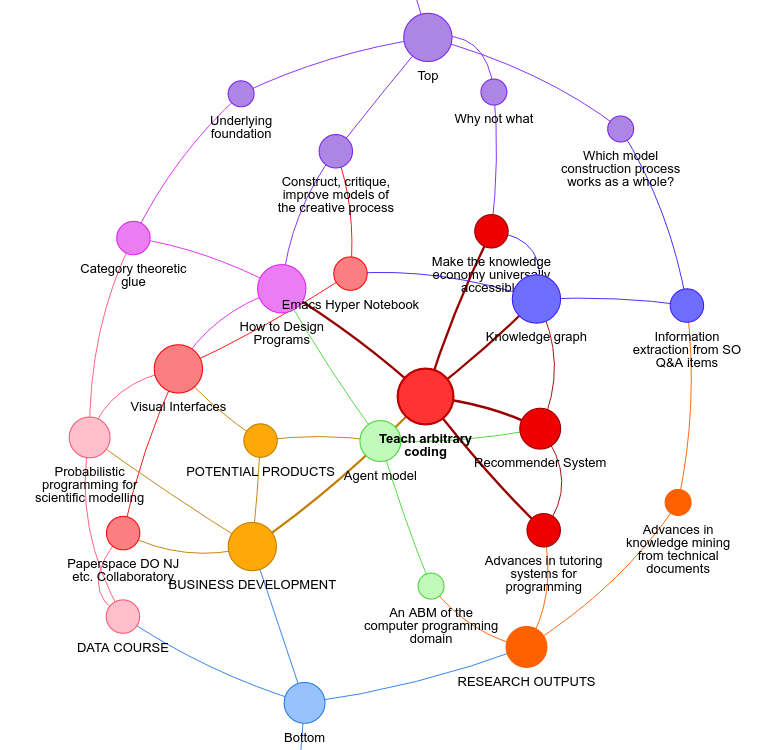
\includegraphics[width=\textwidth]{org-roam-server-3oct2020.png}
\caption{Network view}
\end{figure}

\subsection{Downstream}
\label{sec:org32a9201}
What do our potential users look like?
\subsection{Consulting clients}
\label{sec:orgca41ce5}
We discussed the idea of doing consulting for clients who are
interested in using scientific models.

\emph{Play through again as a consulting client}
\subsection{Scientific software developers}
\label{sec:orgfc5c842}
We imagine some software developers consuming “tutorial” content we
produce, and improving their skills and abilities as a result.

\emph{Play through again as a consulting client}
\subsection{Automated tutoring system users}
\label{sec:org0ca358e}
We imagine some students using AI software we develop.  In some cases
they could be “students”.  In other cases, they could already be
professional developers.
\subsection{Programmers}
\label{sec:orgdbe9fe7}
We imagine any programmer having some use for our tools.  “B2D”
(Business to Developer) is an emerging category of enterprise where we
can do interesting things.
\section{Organisational infrastructure}
\label{sec:orge4802fc}
This section is mildly-technical appendix.  It looks at our
organisational infrastructure itself, including simple things like the
technologies we use for communication, and more involved things like
“how we communicate” more broadly.  (This is a good candidate for
splitting off into its own separate wiki, if for no other reason than
that it takes up a lot of space in the generated PDF.)

\subsection{Schedule and activities}
\label{sec:org27dfd6d}

Presently we are meeting 20 minutes a day at 4PM UK time, 11AM
Eastern, on Discord for a “coffee chat”.

Previously we tried to maintain a schedule of longer meetings (UK
evenings):

\begin{itemize}
\item \textbf{Monday}: Seminar
\item \textbf{Wednesday}: Workshop
\item \textbf{Friday}: Studio
\end{itemize}

That seemed to be too many meetings.  Whatever we do about regularly
scheduled meetings, we might want to look at how to best pursue of
\textbf{*topics of mutual interest} such as:

\begin{itemize}
\item \textbf{Readings} on rewriting rules and production systems, and higher-dimensional graph-like things
\item \textbf{Business development} around open source, knowledge management, etc.
\item \textbf{Reviewing} the value add of Wiki ways of thinking and working, which we have a pretty broad range of experience with
\item \textbf{R\&D} around ‘lenses’ in ACT: structure for bi-directional transformations, to enable changes in a projection
\end{itemize}

So far, this Roadmap has gathered information on some of the topics
that have been discussed, but not all of the things that we could see
ourselves working on together.

As another activity we may want to get scheduled one or more sessions
focused on business stuff.

\subsection{Project orientation}
\label{sec:orgca056dc}

Some of this will be different depending on whether we think of this
as a “business”, or as “a business of some specific nature”: primarily
centring on “who does this business do business with?”

\begin{itemize}
\item \textbf{Status} - where is the project right now?
\begin{itemize}
\item Right now \emph{this overall project} is in a “project development” mode.
\item What are the (multiple) \emph{success indicators} or \emph{proof points} or \emph{failure indicators} for each of the projects? (E.g., going to the casino with \$20, you might quit when you get below \$10, you might leave when you get above \$50.) E.g., need of customers for X, our credibility in X?
\item For the various sub-projects: one relevant thing is “how long is it before thing is likely to make money?” (AKA, “Cross-over.”) Or “what else is needed for this to make money?”
\item In particular: maybe take a couple months to see how things are going with a given sub-project? This gives evidence of what we can produce when we work together. We might then ask, who else would care to pay for this?
\item We have listed 4 active projects (\url{https://miro.com/app/board/o9J\_kmPNvaQ=/}); maybe the blog is another one.
\end{itemize}
\item \textbf{Roles and Responsibilities} - \emph{who is handling the standard project roles, and what are they responsible for doing?}
\begin{itemize}
\item Each individual sub-project is likely to have different requirements (e.g., some may need 2 people, some will need 1, etc.)
\item If there’s more than one person involved it becomes a parallel architecture
\end{itemize}
\item \textbf{Goals} - \emph{What will this project achieve?}
\begin{itemize}
\item “If I do something valuable, the money will come later.”
\item Some of them we might be willing to take the risk of investing time and energy based on whether it looks directly useful to us.
\item Some, like a course, we may need the information about whether it’s likely to be taught.
\item Some could become a paper or the building block of a business: these can be small demo projects.
\item Alternatively, in a consulting mode, our role becomes understanding customer goals and helping rationalise work to fulfil them.
\end{itemize}
\item \textbf{Resource Requirements} - \emph{What (people, money, things) are needed to accomplish this project?  Where do they come from?}
\begin{itemize}
\item We each individually need some money, but it’s not totally clear that the \emph{company} needs some money.
\item If we wanted to replace any one of us with an employee, then we’d have to have some funding source.
\item If the number of person-hours for the goal is quite high, then it’s unlikely for the goal to be achieved without funding.
\item E.g., what would we need to be able to do consulting?
\end{itemize}
\item \textbf{People} - \emph{Who are the people working on this project? Who can I ask for more information? How can I best get in touch with them?}
\begin{itemize}
\item If we were to be doing consulting, then it becomes about serving specific customer needs.
\end{itemize}
\item \textbf{Approach} - \emph{What is the overall strategy for accomplishing this project?}
\begin{itemize}
\item Whatever we choose (e.g., consulting vs product development) we should choose it based on some data and analysis.
\item Wherever we are now, the question is what’s needed to move ahead.
\end{itemize}

\item \textbf{Workplan and Timeline} - What are the specific tasks needed to accomplish our goals? When might they happen? Who / what / when (in agile, we specify two).
\begin{itemize}
\item Joe needs some job soon!
\item To do consulting we’d need to figure out customer need and credibility
\item To make progress on the AI directions we need some version of all the things up and running!
\end{itemize}
\item \textbf{Communication Norms} - how have the project participants agreed to stay in touch? what, where and how often are regular meetings? Special ceremonies?
\begin{itemize}
\item In 2 months we’ll have 2 more months of experience.  So we could then assess things.
\item In advance of that, we might start to understand the expections about how we would gather the data.
\item It should be pretty much fun, and if it’s not we’re kind of doing it wrong?
\item On an ongoing basis we should be able to check whether what we’re doing is effectively addressing the goals we have
\end{itemize}
\item \textbf{Sponsor} - \emph{the person who requires the output of the project and has allocated the resources for it (aka Customer in agile)}
\begin{itemize}
\item So far we’re all sponsoring our own work on sweat equity
\item While also trying to be helpful \& respectful to each other
\item EF was the sponsor at one time
\item Joe provided chips and dip but the event was strictly BYOB\ldots{} as long as we’re here we’ll make the best out of.  Polka time!
\end{itemize}
\item \textbf{Project Manager} - the person responsible for the drumbeat and tempo of the project, and for its administrative details, including good project management hygiene
\item \textbf{Lead} - the person responsible to the Sponsor for making sure the project is accomplished and to the Team for making sure they are able to accomplish the project
\begin{itemize}
\item Ray: project to build bridges between participants (e.g., systems bio, category theory, stats); this is related to the “transdisciplinary design” course
\item Joe: I’m less technically sophisticated
\end{itemize}
\item \textbf{Team} - people working on the project
\begin{itemize}
\item Everyone will have some constraints (like need \$40K per year if it takes more than 20 hours per week)
\end{itemize}
\end{itemize}

\subsubsection{Project Management Hygiene}
\label{sec:org376a52a}

\begin{itemize}
\item set SMART goals (Specific, Measurable, Achievable, Relevant and Time-based)
\begin{itemize}
\item (See also: \emph{Coaching and Mentoring}.)
\end{itemize}
\item understand tasks required to accomplish goals, then set realistic timeline
\item create project plan in wiki
\item regular, frequent check-ins to iterate plan (goal, priorities, etc.) if necessary
\item after-action reviews at the end of project, including reflection/writeup of positives and deltas
\item experienced, well-oiled teams requires less strict project management hygiene
\item new, less-organized, or heterogenous teams require more attention to careful project management hygiene
\end{itemize}

\subsubsection{{\bfseries\sffamily STARTED} Review the Exp2Exp backlog to decide which things are wontfix, what other categories need to be created, etc.}
\label{sec:org4eb1b4b}
I can browse these locally with \texttt{C-c R e}.

\subsubsection{{\bfseries\sffamily BACK} Make a list of actual topics of interest}
\label{sec:org6c549be}
If we were just doing “content production” we might think of a list of
chapters to write, or podcasts to produce. However, maybe those ways
of thinking and working don’t apply comfortably here.

\subsubsection{{\bfseries\sffamily BACK} Make a project analysis of active projects}
\label{sec:org2710885}
This could refer to Peter Kaminski’s ``\hyperref[sec:orgca056dc]{Project orientation}'' described in \hyperref[sec:orge4802fc]{Organisational infrastructure}.

\subsection{Technology}
\label{sec:orgc37247b}

Does \url{https://github.com/orgs/exp2exp/projects/1} conflict, replace, or
serve a different function compared with Org mode agenda items?

\subsubsection{{\bfseries\sffamily DONE} Figure out Github project(s) vs Org todos\hfill{}\textsc{joe:cameron}}
\label{sec:org99c8fa0}

We won’t use Github stuff right now.  That’s better for dealing with a
public-facing contribution workflow when we have actual open source
things running with contributors.

\subsection{Discord server}
\label{sec:orge100869}
We set up a Discord server that we’re using for our meetings.  This
invite link should not expire: \url{https://discord.gg/pArjt4p}

(We also have a Zulip server set up, but currently we’re using it
less.)
\subsection{OBS recordings}
\label{sec:org1b47ff5}
We talked about creating asyncronous recordings (screencasts,
audio). We also talked about possibly putting the audio recordings
into a threaded voice mail forum, but that's a somewhat different
application.

\subsection{Code sharing platform}
\label{sec:org8675f1a}
For now we have a Github organisation (\url{https://github.com/exp2exp}), as
well as a separate repo that contains these Org Roam notes, among
other things.  This could potentially be improved or upgraded in
various ways.

\subsubsection{Comments}
\label{sec:org3633f35}

\begin{itemize}
\item Nextjournal is interesting
\item It's like a Jupyter notebook
\item It's like Org Bable so you can run code in any language within the same environment
\item If I need to add a bash cell to a Julia notebook, it adds a kernel as needed at the run time
\item If I install a bunch of libraries, and save the current environment in a docker container, you can import it
\item It doesn't yet have an easy way to make an app?
\end{itemize}

\subsubsection{What if you had a browser based version of Org Bable?}
\label{sec:org0c9f535}

\begin{itemize}
\item You could have your notebook, backed by the ability to use Emacs
\end{itemize}

\subsubsection{Examples}
\label{sec:org115f9c9}

\begin{itemize}
\item Setting up a data science experiment
\item Wadler et al. course in Agda in NextJournal
\item But you can't easily treat this as ‘Org Roam’ (no bi-directional things)
\end{itemize}

\subsubsection{Next evolution}
\label{sec:orgc213fdf}

We need a basic code sharing platform to get to work.  The next
evolution might look like what we’ve been calling the “Emacs Hyper
Notebook”?  However, some contributors are not interested in using
Emacs for everything.  And we can’t assume that users would be
interested in it either!
\subsection{Wiki}
\label{sec:org675d604}
The public facing version of these notes is available on a simple web
interface, created by firn: \href{https://exp2exp.github.io/}{https://exp2exp.github.io/}. This mirrors
the contents of our Org Roam directory.  Editing is explained below.

We can also view the contents of Org Roam in a linear form as PDF
document\ldots{} or view the currently active tasks using Org Agenda.  In
the future we may want to have several different “upstream” locations,
based on several different small-scale wikis, all feeding into this
one location.  That’s not hard to set up.  Contents can also be
browsed in a graphical form either with the built in \texttt{org-roam-graph}
functionality, or by installing Org Roam Server and running
\texttt{org-roam-server-mode}.

We can potentially improve on all of this further, bulding something
like Metacademy.  For now, we describe how to use this simple Org Roam
based wiki.

\subsubsection{Access}
\label{sec:org0e0c9bf}

Obtain the sources by cloning the repo at \href{https://github.com/exp2exp/exp2exp.github.io}{https://github.com/exp2exp/exp2exp.github.io}.

\begin{verbatim}
git clone git@github.com:exp2exp/exp2exp.github.io.git
\end{verbatim}

(See below for an alternative.)

\subsubsection{Mob branch on repo.or.cz}
\label{sec:orgab6b465}

We’re mirroring the repo to an environment that allows anonymous
commits (without need for further permissioning).  If want to
contribute anonymously, info on that is here: \href{https://bit.ly/2EQRHEF}{https://bit.ly/2EQRHEF}

You can review commits to the mob branch here: \href{https://repo.or.cz/arxana.git/shortlog/refs/heads/mob}{https://repo.or.cz/arxana.git/shortlog/refs/heads/mob}

\subsubsection{Setup}
\label{sec:org3b32dec}

Install Org Roam if needed (\texttt{M-x package-install RET org-roam RET}).

Subsequently, add this to your Emacs configuration:

\begin{verbatim}
(require 'org-roam)
(setq org-roam-directory (concat "/home/"
                          (getenv "USER")
                          "/exp2exp/"))
(setq org-roam-completion-system 'helm)
(define-key org-roam-mode-map (kbd "C-c n l") #'org-roam)
(define-key org-roam-mode-map (kbd "C-c n f") #'org-roam-find-file)
(define-key org-roam-mode-map (kbd "C-c n b") #'org-roam-switch-to-buffer)
(define-key org-roam-mode-map (kbd "C-c n g") #'org-roam-graph)
(define-key org-mode-map (kbd "C-c n i") #'org-roam-insert)
(org-roam-mode +1)
\end{verbatim}
\subsubsection{Bonus feature: org-roam-checkout}
\label{sec:org5781f9a}

If you regularly use your own separate Org Roam setup, you can use
this simple context switcher to move between the two.  Keep track of
the various separate Org Roam installations with \texttt{org-roam-library}
and then switch between them interactively with \texttt{org-roam-checkout}.

\begin{verbatim}
(defvar org-roam-library `(,(concat "/home/" (getenv "USER") "/exp2exp/")
                           ,(concat "/home/" (getenv "USER") "/org-roam/")))

(defun org-roam-checkout ()
  (interactive)
  (let ((ctx org-roam-directory))
    (if (eq (length org-roam-library) 1)
        ;; Still go ahead and set the variable in this case!
        (progn (setq org-roam-directory (car org-roam-library))
               (message "You only have one choice for org-roam-directory defined."))
      (let ((lib (completing-read "Choose a volume: " org-roam-library)))
        (when lib
          (setq org-roam-directory lib))))
    ;; assuming the user changes context, let’s also prompt them
    ;; to choose a new file in that context
    (when (not (eq ctx org-roam-directory))
      (org-roam-find-file))))
\end{verbatim}

\subsubsection{Interaction}
\label{sec:orgb636c49}

Use the \texttt{C-c n f} keyboard command to add new disconnected nodes to
the graph, or use \texttt{C-c n i} to create a page and insert a wiki-style
link, like \texttt{[[New Page]]}. Follow links with \texttt{C-c C-o}. Display the
graph structure with \texttt{C-c n g}.  It may be necessary to run \texttt{M-x
org-roam-db-build-cache} to get the graph to match reality.  Add and
commit new or modified files with git, along with \texttt{org-roam.db}, and
push them to the repo.

\subsubsection{Tags}
\label{sec:org515f293}

Some of the nodes have \texttt{\#+roam\_tags} set:

\begin{center}
\begin{tabular}{ll}
\textbf{code} & \textbf{meaning}\\
\hline
HL & High level\\
CDN & Can do now\\
LRD & Longer R\&D cycle\\
HD & Has dependencies\\
RR & Research Review\\
RO & Research Output\\
OTS & Off the shelf\\
SH & Stakeholder\\
AN & Annex\\
\end{tabular}
\end{center}

Some of the files also have a \texttt{\#+CATEGORY} set.

\subsubsection{Pairing}
\label{sec:org500b8b9}

For syncronized browsing and editing with \href{https://github.com/tjim/lockstep}{lockstep.el}:

\begin{verbatim}
ssh pair@178.79.174.58
PW: <ASK JOE FOR THE PASSWORD>
emacsclient -a '' -t
M-x lockstep
\end{verbatim}

To open up a real-time collaboration (with multiple cursors), use
\href{https://code.librehq.com/qhong/crdt.el}{crdt.el}, first to serve the buffer:

\begin{verbatim}
M-x crdt-serve-buffer
\end{verbatim}

And then, from your client, to connect:

\begin{verbatim}
M-x crdt-connect
\end{verbatim}

\subsubsection{Linearizing}
\label{sec:org5a4390b}
To turn this map into something we can reliably use, let’s try to
linearize it.

To downsample from Org Roam (save as \texttt{\textasciitilde{}/bin/roam2org.sh} and make it
executable):

\begin{verbatim}
#! /bin/bash

emacs --batch -l ~/bin/downsample-org-roam.el --eval "(combine-files)" "$@"
\end{verbatim}

Here are the working parts (save as \texttt{\textasciitilde{}/bin/downsample-org-roam.el}):

\begin{verbatim}
(defun downsample ()
  "Process an Org Roam buffer for inclusion in a standard Org file.
Changes title to header, and increase indentation of existing headers.
Changes file links to internal links."
  (if (looking-at "^#\\+TITLE:")
      (replace-match "*"))
  (forward-line 1)
  (if (looking-at "^#\\+roam_tags:\\(.*\\)")
      (replace-match ":PROPERTIES:
  :tag:\\1
  :END:"))
  (while (re-search-forward "^\\*" nil t)
    (replace-match "**"))
  (goto-char (point-min))
  (while (re-search-forward "\\[\\[file:\\([^]]*\\)\\]\\[\\([^]]*\\)\\]\\]" nil t)
    (replace-match "[[*\\2][\\2]]"))
  (buffer-substring-no-properties (point-min) (point-max)))

(defun combine-org-roam-files (&rest args)
"Combine a list of files, specified as ARGs.
The files are to be found in `org-roam-directory'."
  (apply #'concat
         (mapcar (lambda (file)
                   (save-window-excursion
                     (find-file (concat org-roam-directory file))
                     (let ((contents (buffer-substring-no-properties (point-min)
                                                                     (point-max))))
                       (with-temp-buffer (insert contents)
                                         (goto-char (point-min))
                                         (downsample)))))
                 (or (car args) (nthcdr 5 command-line-args)))))
\end{verbatim}

\subsubsection{Backlog}
\label{sec:orgc7dfda6}
Part of the idea with a backlog is to go from most-doable, starting
with work in progress, to least-doable and potentially vague.  Here,
then, is one approximate linearization that may or may not meet that
description!

Note, this is duplicated in the index file, probably for sanity we
should pick one and automate the derived version from there!

\begin{verbatim}
(defvar files-to-combine
'("20200810131435-hyperreal_enterprises.org"
"20200810132653-top.org"
"20200905124558-why_not_what.org"
 "20200909195629-teach_arbitrary_coding.org"
 "20200810135851-how_to_design_programs_with_if.org"
"20200905124405-construct_critique_improve_models_of_the_creative_process.org"
  "20200905125342-emacs_hyper_notebook.org"
  "emacs_jupyter_remote_debugging.org"
"20200905125023-which_model_construction_process_works_as_a_whole.org"
 "20200905131027-information_extraction_from_so_q_a_items.org"
"20200905131918-knowledge_graph.org"
"20200905124432-underlying_foundation.org"
 "20200905125713-category_theoretic_glue.org"
 "20200905131656-probabilistic_programming_for_scientific_modelling.org"
"20201003205523-potential_products.org"
 "20200905130423-agent_model.org"
 "20200817172825-recommender_system.org"
 "20200810135457-visual_interfaces.org"
 "20200814203551-data_course.org"
 "20200905132603-paperspace_do_nj_etc_collaboratory.org"
"20200814210243-business_development.org"
"20200905134325-research_outputs.org"
 "20200810135325-advances_in_tutoring_systems_for_programming.org"
 "20200810135403-advances_in_knowledge_mining_from_technical_documents.org"
 "20200905132334-an_abm_of_the_computer_programming_domain.org"
"20200906003704-bottom.org"
 "20201003164408-downstream.org"
 "20201003165500-consulting_clients.org"
 "20201003170312-open_source_developers.org"
 "20201003170333-tutoring_students.org"
 "20201003171011-programmers.org"
"20200810135126-organisational_infrastructure.org"
 "20200810135619-discord_server.org"
 "20200811185435-obs_recordings.org"
 "20200814193042-code_sharing_platform.org"
 "20200912223428-wiki.org"
 "20201003164100-forum.org"
 "20200814195259-blog.org"
"sfi/sfi.org"
 "sfi/gather_data_via_stack_exchange_apis.org"
 "sfi/argumentation_theoretic_analysis.org"
 "sfi/process_model_analysis.org"
 "sfi/ml_nlp_bootcamp.org"
 "sfi/initial_ml_baseline_e_g_match_q_a.org"
 "sfi/hierarchical_ml_for_content_extraction.org"
 "sfi/active_inference_bootcamp.org"
 "sfi/agent_modelling_and_sandbox_setup.org"
 "sfi/curate_koans_and_develop_solver.org"
 "sfi/study_with_crowdsourced_exercises.org"
 "sfi/study_with_agent_written_questions.org"
 "sfi/publication_ijcai.org"
)
"An ordered list of files to combine in our export.
This is where the order of presentation in the downstream org file
and derived PDF is defined.")
\end{verbatim}

To combine the files, run:
\begin{verbatim}
(combine-org-roam-files files-to-combine)
\end{verbatim}

To get the indicative nesting (shown by spaces above) to be replicated
at the org level, run the following at the top of the exported
compilation:

\begin{verbatim}
(defun indent-org-roam-export ()
  "Utility function to increase indention for selected trees."
  (org-map-entries (lambda ()
                     ;; don’t demote the top level items and their sub-items
                     (let ((tag (org-entry-get nil "tag")))
                       (if (and tag (string= (car (split-string tag)) "HL"))
                           (progn (org-end-of-subtree)
                                  (setq org-map-continue-from (point)))
                         (org-do-demote))))
                   nil 'file))
\end{verbatim}

Lastly, to rebuild the PDF, all of this can be done with one swift
action.

\begin{verbatim}
(defun rebuild-org-roam-pdf ()
  "Build an org file and PDF compiling `files-to-combine'."
  (interactive)
  (save-excursion (find-file (concat org-roam-directory
                                     "/manual/combined.org"))
    (goto-char (point-min))
    (search-forward "# IMPORT")
    (let ((beg (point)))
      (delete-region (point) (point-max))
      (insert "\n" (combine-org-roam-files files-to-combine))
      (goto-char beg)
      (indent-org-roam-export)
      (org-latex-export-to-pdf))))
\end{verbatim}

\subsubsection{Publishing to the web}
\label{sec:org64c8e50}

Publishing with Firn is simple:

\begin{verbatim}
firn build
\end{verbatim}

Then commit and push.

\subsubsection{Reviewing progress}
\label{sec:org1a1857e}

Something like the following should be all that’s get a high-level
overview of progress on active tasks, sourcing information directly
from the Org Roam files.  Add the following to your emacs
initialisation script (e.g., \texttt{\textasciitilde{}/.emacs}), evaluate it, and then run
\texttt{C-c r} to load up the fun.  This may not be the perfect presentation
yet but it gives an idea.

\begin{verbatim}
(setq org-todo-keywords
      '((sequence "TODO" "STARTED" "BLOCKED" "BACKBURNER" "FROZEN"
                  "|" "DONE" "DEFERRED" "WONTFIX")))

(setq org-agenda-sorting-strategy '((todo todo-state-down category-down)))

(setq org-agenda-files '("~/exp2exp/"))

(defun org-scrum-board ()
  (interactive)
  (org-todo-list "TODO|STARTED|BLOCKED|BACKBURNER|FROZEN|DONE|DEFERRED|WONTFIX"))

(global-set-key (kbd "C-c r") 'org-scrum-board)
\end{verbatim}

This view can then be further filtered by regexp (e.g., your name) by
pressing \texttt{=}.

\subsubsection{Notes about exporting things with Firn}
\label{sec:org4c7c0e2}

In regular Org mode, it’s possible to \href{https://superuser.com/questions/726201/how-can-i-apply-easy-formatting-to-org-mode-blocks}{define your own blocks} which
then export to a div with the given block name:

\begin{monoblock}
This is some text.
\end{monoblock}

With Firn/Orgize, it seems these blocks aren’t currently exported.
However, examples are exported?  Maybe not.

\begin{verbatim}
This is some text.
\end{verbatim}

\subsubsection{{\bfseries\sffamily DONE} Package downsamping code separately\hfill{}\textsc{joe}}
\label{sec:orgc219a7c}
\subsubsection{{\bfseries\sffamily WONTFIX} Update the repo instructions to reference this file\hfill{}\textsc{joe}}
\label{sec:org6639b4b}

\subsection{Forum}
\label{sec:orgb61a99d}
We talked about using Wikum as a forum, because we liked the idea of a
workflow based on summarising discussions. There’s now a demo instance
set up that we can use, here:

\url{http://wikum.org/visualization\_flags?id=590\&owner=holtzermann17}

\subsubsection{Could we incorporate the ideas directly in Org or Org Roam?}
\label{sec:org72b7a37}

Perhaps we could incorporate some Wikum ideas right into the wiki
here.  The idea would be to treat the top paragraph on each page as a
summary, and then add discussion threads below.  We’d want some system
of tags that indicated whether the summary was validated or now.
(Note the the original WikiWikiWeb did not have separate talk pages!
I don’t know if they practiced robust summarisation, either.)

\begin{enumerate}
\item REMARK\hfill{}\textsc{joe}
\label{sec:org627f701}
This is an “inline task,” via \texttt{(require 'org-inlinetask)}.  There
doesn’t seem to be support for nested or threaded tasks, but maybe we
would have use for non-threaded forum discussions at the end of any
page in the Wiki.  Incidentally, for those curious, the formatting of
the \LaTeX~export is controlled by
\texttt{org-latex-format-inlinetask-function}.
\item END
\label{sec:org9557007}
\end{enumerate}

\subsubsection{{\bfseries\sffamily BACK} What might our summarisation workflow look like?}
\label{sec:org08e07fc}
Since we’re pretty actively updating our \textbf{Discord} and pretty happy
using it, maybe people who are working on Active Projects would be
willing to summarise on the wiki, say, weekly?  And contribute to a
monthly group blog post?
\subsection{Blog}
\label{sec:org098f971}
For now we’re just maintaining a \emph{blog roll} rather than one shared blog

\begin{quote}
Zans: \emph{If I implemented as I read things, it would be a pretty interesting blog. There could be a huge market of people interested in following this, this would give a pool of people who know who we are. This is a nice goal b/c it doesn't focus on the product\ldots{} but it's a deliverable, made up of smaller deliverables, and a concrete benefit.}
\end{quote}

\subsubsection{Blog roll}
\label{sec:org5e47cb5}

Some of us are writing blogs.

\begin{itemize}
\item \href{https://exp2exp.github.io/updates}{Updates on Exp2Exp} by Joe Corneli
\item \href{https://prodg.org/blog}{Prodg.org} by Deyan Ginev
\item \href{https://zaeph.net/posts/}{Zaeph.net} by Leo Vivier
\item \href{https://exp2exp.github.io/erg}{Emacs Research Group} meeting notes
\end{itemize}

\subsubsection{Blog roll: Others}
\label{sec:orga58b335}

Here are some people with related interests.

\begin{itemize}
\item \href{https://sachachua.com/blog/}{Sacha Chua} maintains a great Emacs blog and newsletter
\item \href{https://weakty.com/chronolog}{Weakty.com} by T Sloane, the primary developer of Firn
\item \href{https://lyderic.origenial.fr/}{Lydéric's Digital Garden} by Lydéric Dutillieu, Clojure programmer, Paris
\item \href{https://doubleloop.net/}{Double Loop.net} by Neil Mather
\end{itemize}
\end{document}